\documentclass[a4paper]{article}
\usepackage[english]{babel}
\usepackage[T1]{fontenc}
\usepackage[utf8]{inputenc}
\parindent 10pt
\usepackage[tbtags]{amsmath}
\usepackage{amssymb, amsthm, mathtools, physics}
\usepackage{siunitx}
\usepackage{mhchem}
\usepackage{empheq}

\usepackage{circuitikz}

\ctikzset{bipoles/thickness=1.2}

\usepackage{pgfplots}
\usepackage{float}
\pgfplotsset{compat=1.15}

\usepackage{lmodern}
%\usepackage{tgbonum}
%\usepackage[T1]{fontenc}

\usepackage[margin=1in, top=1.25in, headheight=2\baselineskip, headsep=\baselineskip]{geometry}
\usepackage{fancyhdr}
\usepackage[pdfusetitle, colorlinks]{hyperref}
\usepackage[shortlabels, inline]{enumitem}
\usepackage{multicol, array}
\usepackage{titlesec}
\usepackage[titles]{tocloft}
\usepackage{xcolor, xpatch, calc}
\usepackage{multirow}
\usepackage{comment}
\usepackage{lipsum}
% \usepackage{indentfirst}
% \usepackage{setspace}



% Grafici
\usepackage{graphicx, booktabs, wrapfig, pdfpages}
\usepackage{pgfplots}
\usepackage{pdfpages} %prova M
\usepackage[framemethod=tikz]{mdframed}
\usepackage[outline]{contour}
\usepackage[ labelfont=bf, labelsep=period, font=small]{caption}
%margin=0.2in
%\usepackage{subcaption}
\usepackage{caption}
\usepackage{subfig}
\usepackage[rightcaption]{sidecap}
\usetikzlibrary{babel, calc, scopes, intersections, angles, quotes, arrows, arrows.meta, backgrounds, shapes.geometric, patterns, shadows, perspective, external}
\tikzset{
	font = {\selectfont},
	frame/.style={thin, dashed, lightgray, line cap=round, rounded corners=5pt}
}
\contourlength{1pt}


% path della cartella delle figure
\graphicspath{{images/}{figs/}}


% --- frontespizio ---

\title{\mytitle}
\author{\myauthor}
\date{\thedate}

	
\newcommand{\mysubtitle}%
	{Study of Timing Measurements}

\newcommand{\myauthor}%
	{Saadallah Shagul, Sibilla Margherita, Vianello Emma - Group 30}
    
\newcommand{\myemail}%
	{{\texttt{shagulraoofsaadallah.saadallah@studenti.unipd.it}} - matr. 2142057\\      
        {\texttt{margherita.sibilla@studenti.unipd.it}} - matr. 2149745\\
	{\texttt{emma.vianello@studenti.unipd.it}} - matr. 2156560}

\newcommand{\thedate}%
	{18 november 2024}

\newcommand{\thesubject}%
	{Physics laboratory}

\newcommand{\firstinstitute}%
	{Universit\`a degli Studi di Padova}

\newcommand{\secondinstitute}%
        {Department of Physics and Astronomy ``G. Galilei''}
    
\newcommand{\shortinstitute}%
	{DFA}

\usetikzlibrary{babel, calc, scopes, intersections, angles, quotes, arrows, arrows.meta, backgrounds, shapes.geometric, patterns, shadows, perspective, external}
\pgfplotsset{compat=1.18} 

% Colori
\definecolor{padovauniversityred}{rgb}{0.8, 0.0, 0.0}
\newcommand{\emphcolor}{gray}

% Tutti i link in grigio
\hypersetup{allcolors=\emphcolor}

% Elenco personalizzazione
\setlist[enumerate, 1]{
	label=\textbf{\emphcolor}{\arabic*.},
	labelindent=\parindent,
itemindent=*,
	ref=\textbf{\arabic*}
}
\setlist[enumerate, 2]{%
	label=\textbf{\color{\emphcolor}(\alph*)},
	itemindent=*,
	ref=\textbf{(\alph*)}
}
\setlist[enumerate, 3]{%
	label=\color{\emphcolor}\roman*.,
	itemindent=*,
	ref=\roman*
}

% Personalizzazione dell'indice
\renewcommand{\cftdotsep}{1}
\renewcommand{\cftsecleader}{\cftdotfill{\cftdotsep}}
%\renewcommand{\cftsecpresnum}{\emphcolor}
\renewcommand{\cftsecaftersnum}{.}
\setlength{\cftsecindent}{25pt}
\renewcommand{\cftsecafterpnum}{\hspace*{25pt}}
\setlength{\cftbeforesecskip}{\baselineskip/2}


% --- Disegno del documento ---



% Colonne
\setlength{\columnsep}{0.5cm}% Separazione tra le colonne

% Disegno dei titoli delle sezioni
\titleformat{\section}[hang]
{\Large\centering\bfseries}
{\thetitle.}{\widthof{\ }}{\Large\color{black}}

% Titolo del documento
\newcommand{\cover}{%
	\thispagestyle{plain}
	\begin{center}
		\Large\textbf{\textcolor{\emphcolor}{\mytitle}} \\
		\LARGE\textbf{\mysubtitle}
		\bigskip
		
		\normalsize\myauthor \\
		\small\myemail
		\medskip
		
		\normalsize\firstinstitute \\ 
		\secondinstitute
		\medskip
		
		\normalsize\thedate \\
	\end{center}%
}


% Tipologie di colonna
\newcolumntype{P}[1]{>{\centering\arraybackslash}p{#1}}
\newcolumntype{M}[1]{>{\centering\arraybackslash}m{#1}}
\newcolumntype{R}[1]{>{\arraybackslash}m{#1}}

% maquillage 
\fancypagestyle{plain}{%
	\renewcommand{\headrulewidth}{0pt}
	
	\fancyhf{}
	\fancyfoot[c]{%
		\begin{tabular}{M{1em}@{}M{2em}@{}M{1em}}
			\textcolor{\emphcolor}{$\boldsymbol{-}$}
			& \thepage &
			\textcolor{\emphcolor}{$\boldsymbol{-}$}
		\end{tabular}
	}
}

% Disegno dell'intestazione e pie' di pagina
\pagestyle{fancy}

\renewcommand{\headrulewidth}{1pt}% riga di separazione intestazione
\xpretocmd\headrule{\color{\emphcolor}}{}{\PatchFailed}% Colore della riga

\fancyhf{}
\fancyhead[l]{%
	\begin{tabular}{@{}R{2.25em}@{}R{\widthof{\shortinstitute\ }}}
		
\includegraphics[height=.25in]{logo.pdf}% simbolo dell'Universita'
		& \shortinstitute
	\end{tabular}
}
\fancyhead[r]{%
	\textit{\thesubject}% Titolo del corso
}
\fancyfoot[c]{%
	\begin{tabular}{M{1em}@{}M{2em}@{}M{1em}}
		\textcolor{\emphcolor}{$\boldsymbol{-}$}
		& \thepage &
		\textcolor{\emphcolor}{$\boldsymbol{-}$}
	\end{tabular}
}

% --- Inizio del documento ---

\begin{document}

	
% --- Frontespizio ---
	
	\phantom{.}\vfill
	\cover
	
%	\begin{center}
%		\rule{.9\textwidth}{0.4pt}%
%	\end{center}
%	\begin{abstract}
%		
%		\medskip
%		\end{abstract}
	\selectlanguage{english} 

	\begin{center}
		\rule{.9\textwidth}{0.4pt}%
	\end{center}
	\selectlanguage{english}
	
	\tableofcontents
	\phantom{.}\vfill\phantom{.}
    
        \thispagestyle{empty}
	\clearpage


\section{Introduction}

\setcounter{page}{1}
In this experiment, in coincidence timing measurements are performed with two different processing systems: first with modular analog electronics (CFDs and TAC), then with a digital equivalent of CFDs. 
The main goal is to study the time resolution $R$ -- defined as the FWHM of the prompt coincidence peak in the time spectrum -- as a function of several parameters of the time peak-off method. 
As for the analog CFDs, the parameters are the external delay and the energy selection, whereas in the digital CFDs also the attenuation fraction and the baseline estimation are varied. 
The second goal is to measure the speed of light by means of time-of-arrival measurements obtained with the analog CFDs and the TAC.

\section{Data analysis, results and discussion}

\subsection{Anode signals}
\hypertarget{2.1}{}
Two organic scintillators mated with PMTs, hereafter referred to as D\#1 and D\#2, were in contact with two opposite faces of a lead brick, which contained and collimated a \ce{^{22}Na} source. 
The detectors could slide on a guide. 
Gamma-ray emissions of the source consist of two 511 keV coincidence photons and one 1275 keV photon for each decay event. The anode signals from the PMTs were observed on the oscilloscope screen. They had negative polarity and different amplitudes, spanning up to $\approx$1 V for both detectors. The pulses corresponding to the Compton edge of 511 keV photons are expected to have intermediate heights, accumulating around a common value. For D\#1 these signals had an amplitude of $\approx$280 mV, a downfall time of $\approx$5.9 ns and a rise time of $\approx$14 ns, while for D\#2 the values were $\approx$360 mV, $\approx$6.7 ns and $\approx$13 ns respectively.

\subsection{Energy calibration}\label{sect: energy calibration}

The anode outputs of D\#1 and D\#2 were connected to CH0 and CH1 of the digitizer, respectively. 
Energy information is contained in the charge of the pulse, i.e. in its area. 
To calibrate the pulses' areas measured by the digitizer in terms of the absolute gamma-ray energy, two 15 minutes files were acquired without imposing the coincidence condition between the detectors: the trigger was set on D\#1 output for the first file and on D\#2 for the second one. 
As expected, the resulting spectra (Fig. \ref{fig: histo calibration d1 d2}, lower x-axis) show two Compton continua each, the first due to the scattering of 511 keV photons and the second created by 1275 keV photons.
\begin{comment}
    
\begin{figure}[H]
  \begin{flushright}
    \hspace{-2 cm}%
    \begin{minipage}[t]{0.6\textwidth}
      \centering
      \hspace{-1.0 cm}
     %  \hspace{0 cm}
      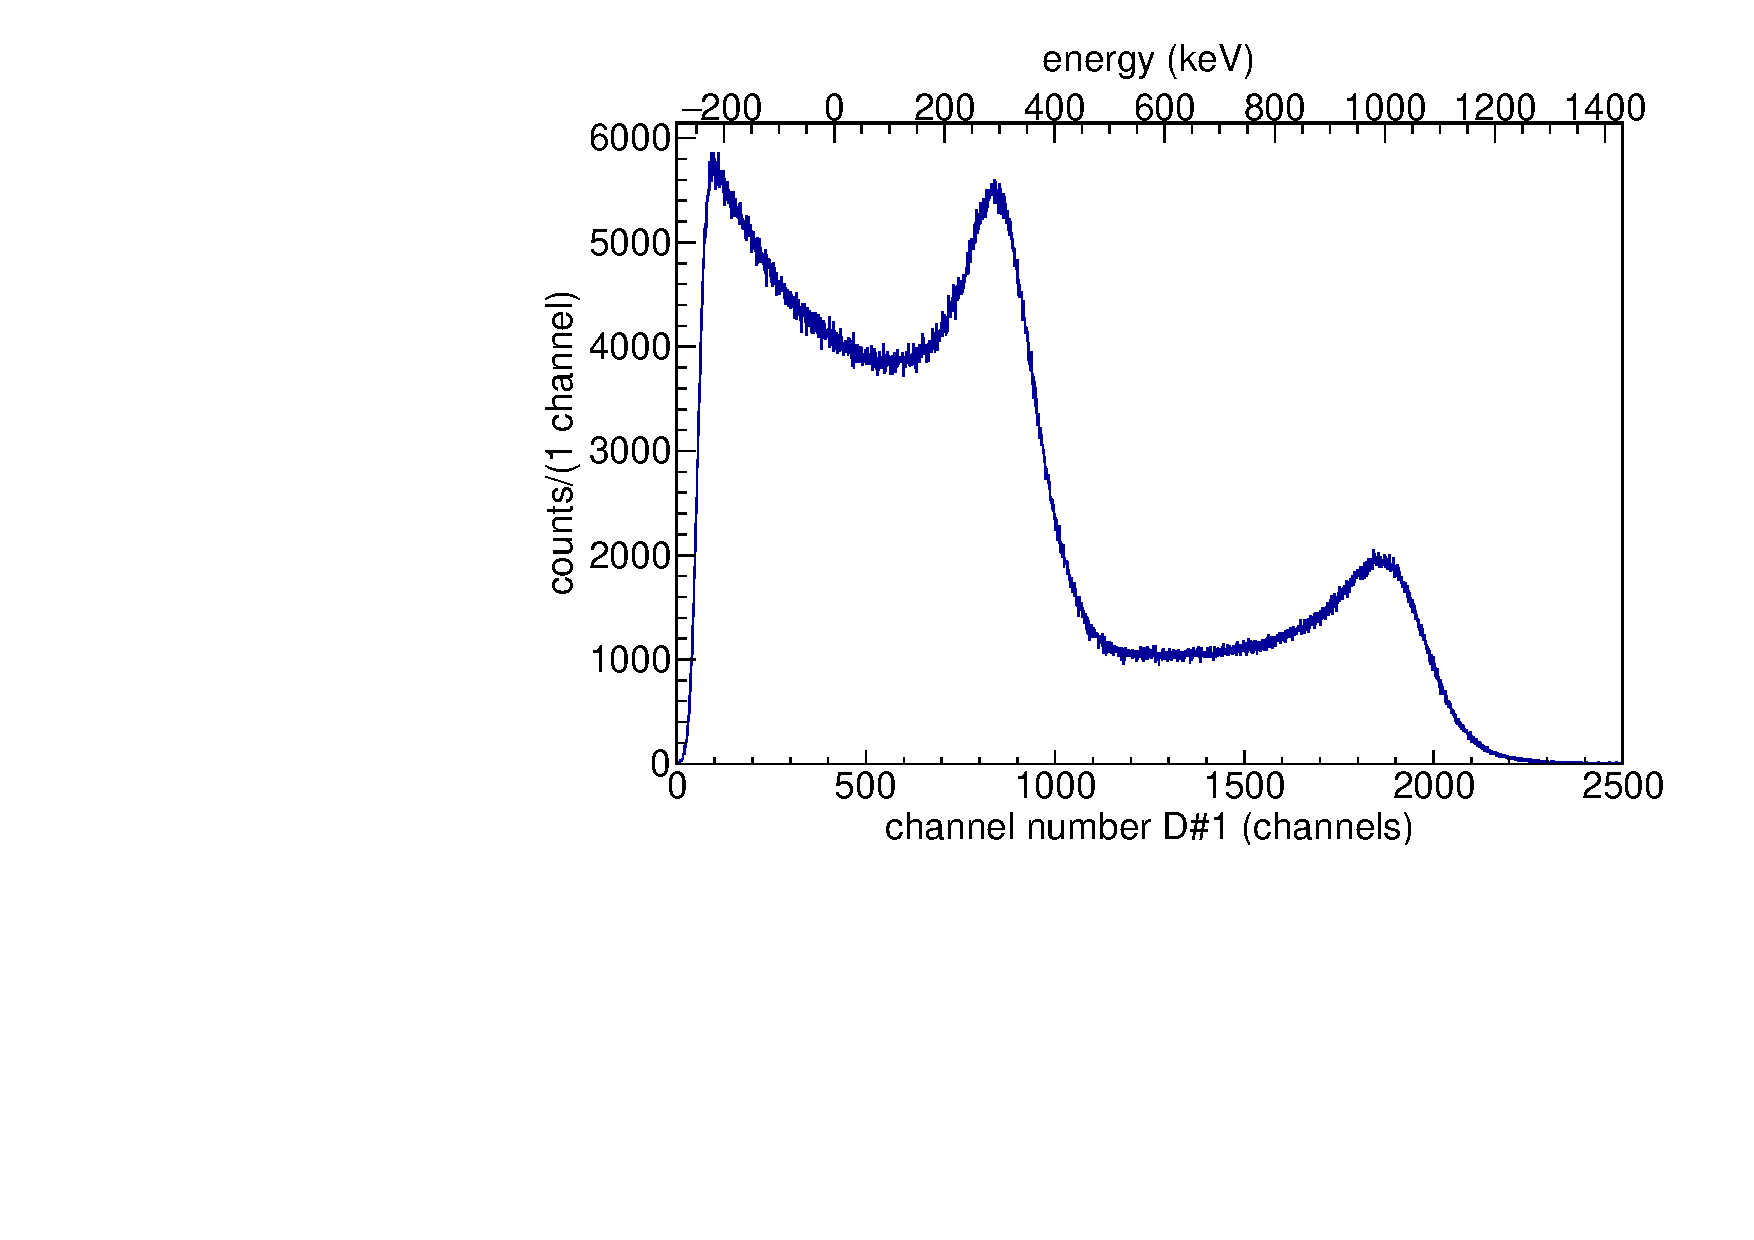
\includegraphics[scale=0.40]{en_cal_figures/ch0_D1_bigger2.pdf}
      \hspace{-1.6 cm}
    \end{minipage}%
    % \hspace{0.5cm}%
    \begin{minipage}[t]{0.6\textwidth}
      \centering
      \hspace{-2 cm}
      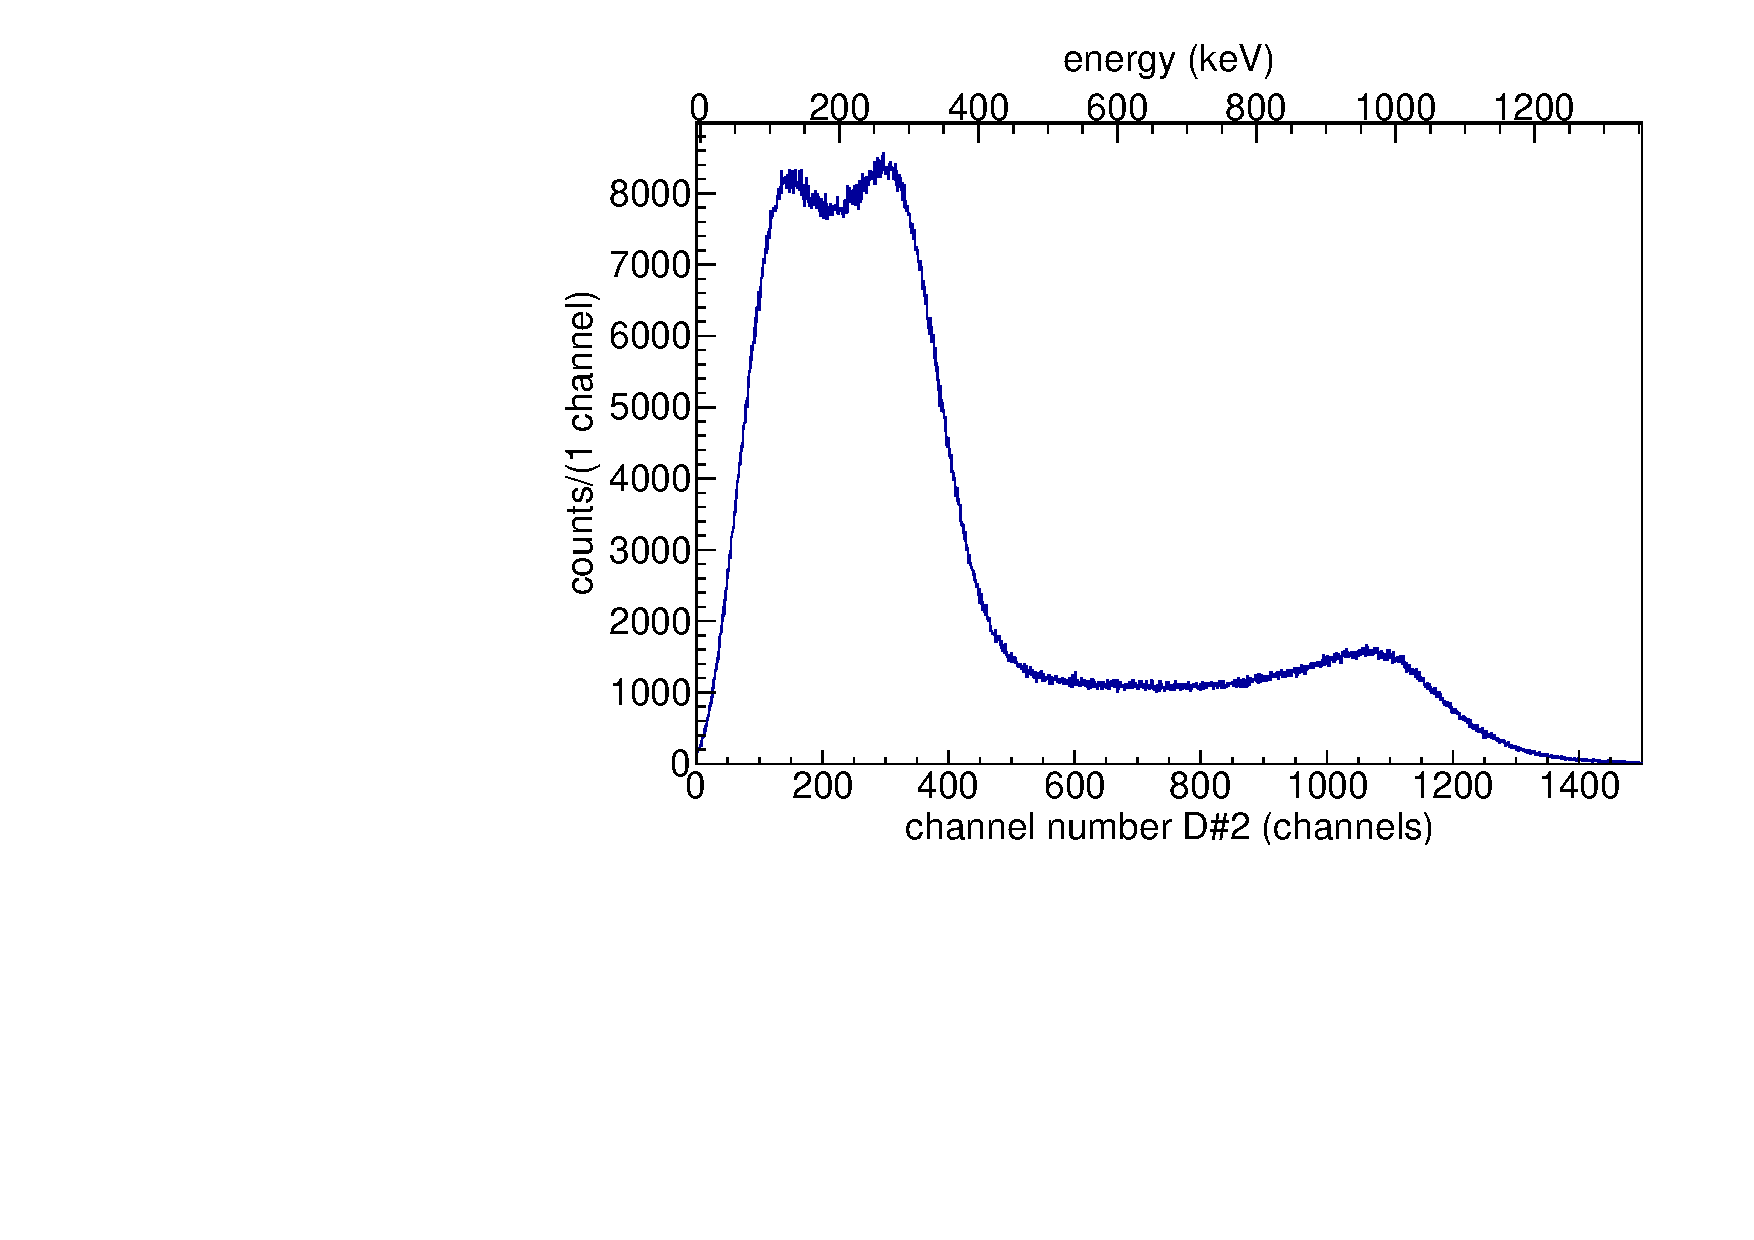
\includegraphics[scale=0.40]{en_cal_figures/ch1_D2_bigger.pdf}
      % \hspace{-1.8 cm}
    \end{minipage}
  \end{flushright}
  \caption{Pulse-height spectra of \ce{^{22}Na} on D\#1 (left panel) and D\#2 (right panel). Upper x-axis represents the calibrated energy. The width of a bin corresponds to $\approx$0.68 keV (D\#1) and $\approx$0.91 keV (D\#2).}
   \label{fig: histo calibration d1 d2}
\end{figure}

\end{comment}

\begin{figure}[H]
    \centering
    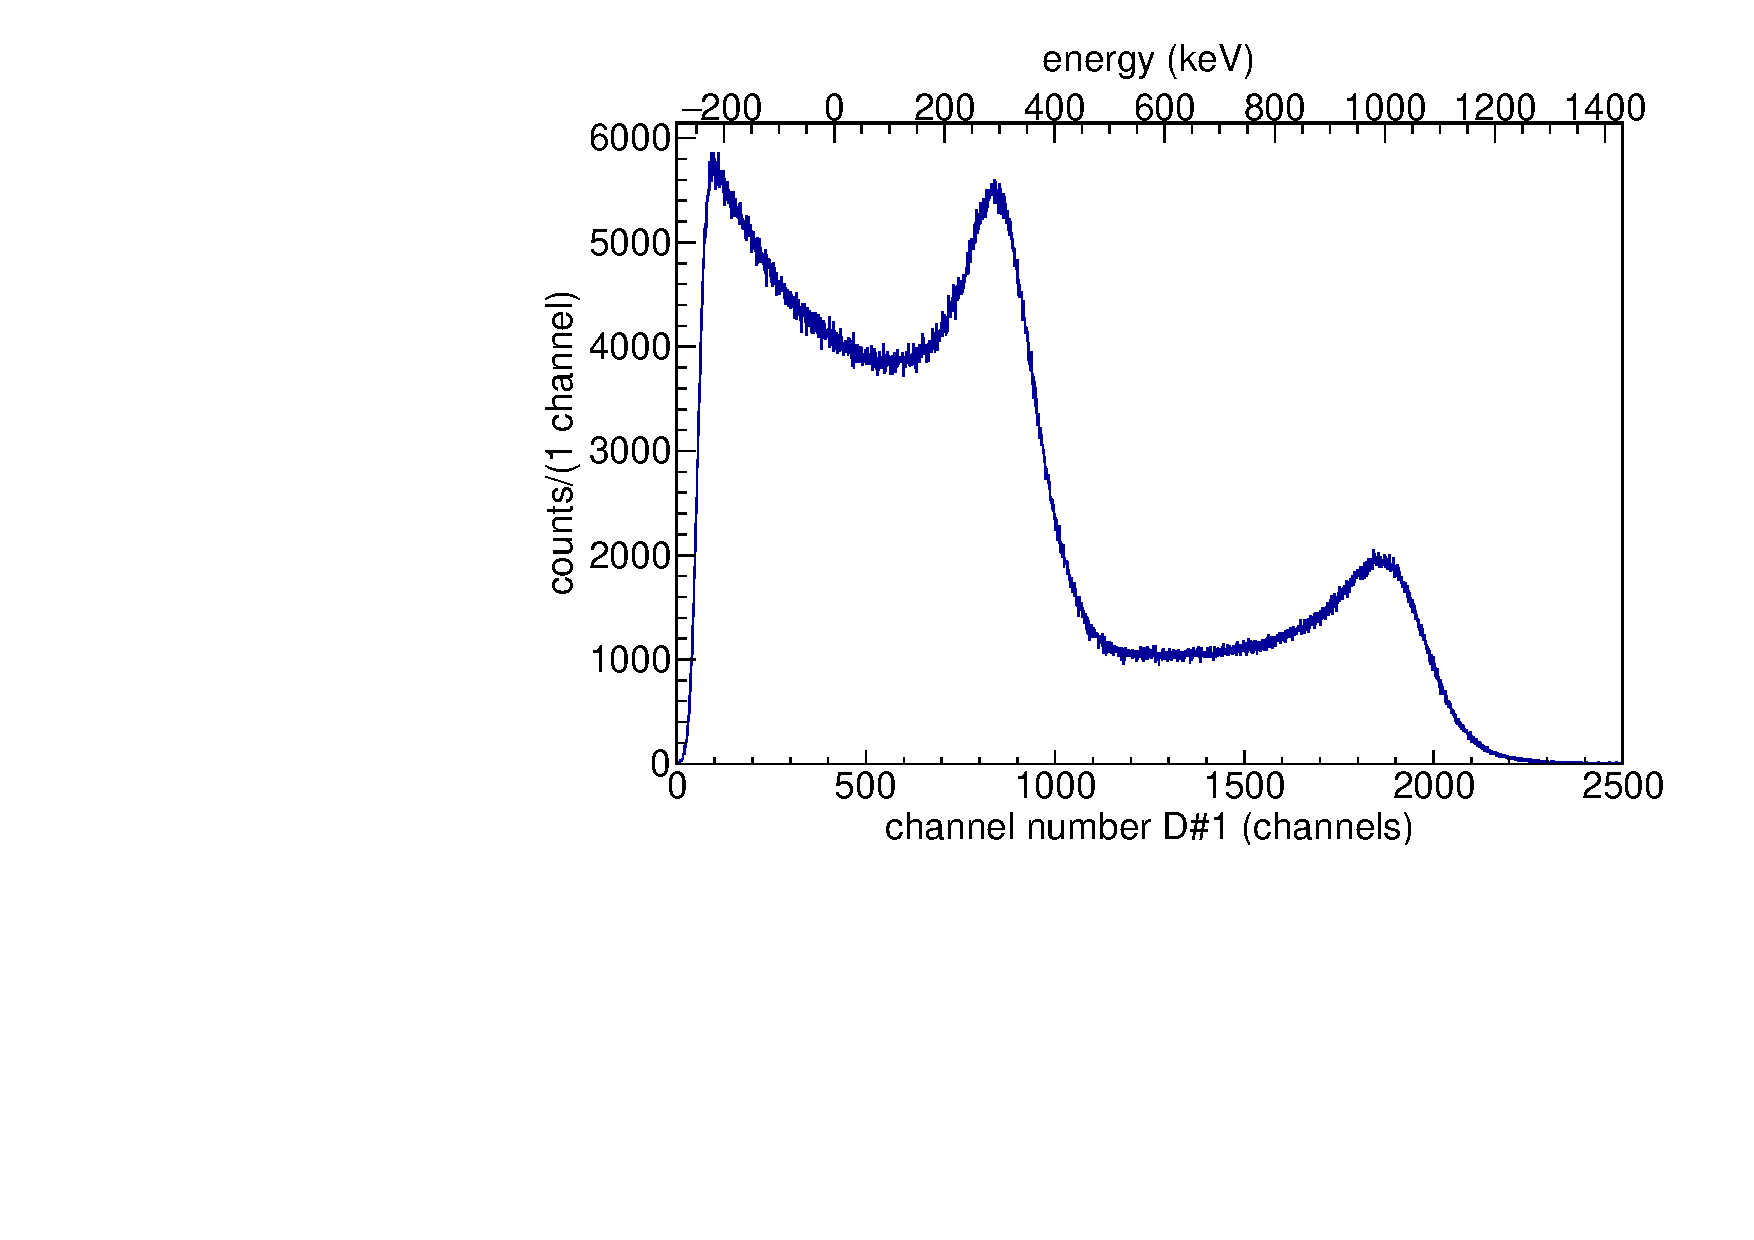
\includegraphics[width=0.5\linewidth]{en_cal_figures/ch0_D1_bigger2.pdf}
    \hspace{-0.5 cm}
    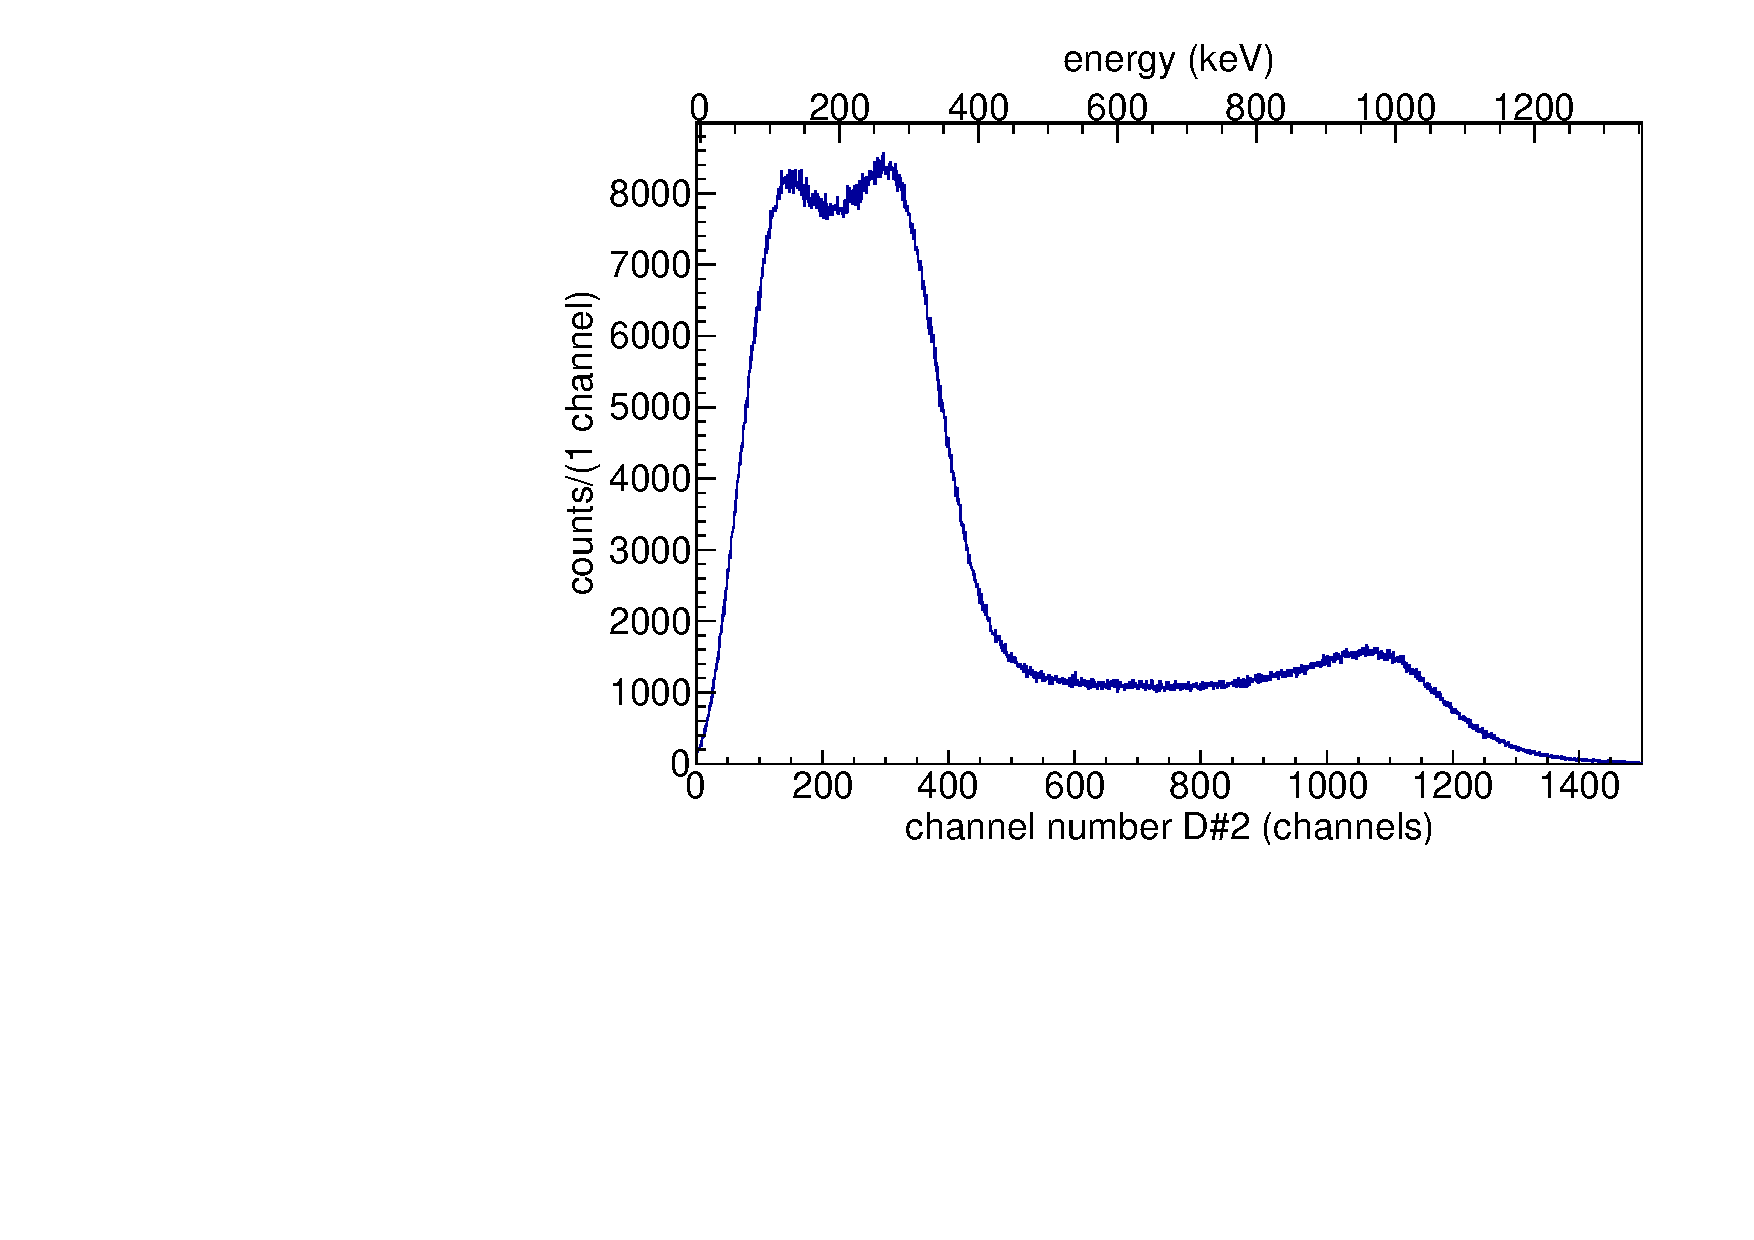
\includegraphics[width=0.5\linewidth]{en_cal_figures/ch1_D2_bigger.pdf}
    \caption{Energy spectra of \ce{^{22}Na} on D\#1 (left panel) and D\#2 (right panel). Upper x-axis represents the calibrated energy.% The width of a bin corresponds to $\approx$0.68 keV (D\#1) and $\approx$0.91 keV (D\#2).
    }
   \label{fig: histo calibration d1 d2}
\end{figure}

Due to the finite pulse resolution of the scintillation detectors, the Compton edge corresponds to an energy value ($E_{\mathrm{CE}}^{\mathrm{shifted}}$) that is lower than the theoretical one ($E_{\mathrm{CE}}$) by a quantity $\Delta E_{\mathrm{CE}}$
\begin{equation}\label{eq: shift of CE}
    E_{\mathrm{CE}}^{\mathrm{shifted}}=E_{\mathrm{CE}}-\Delta E_{\mathrm{CE}}
\end{equation}
To determine the shift $\Delta E_{\mathrm{CE}}$ we used the simulated response functions of Fig. \ref{fig: find Compton shift}, once the \textit{parameter} $\sigma/C$ was known. 
Here $\sigma$ and $C$ are the standard deviation and the mean of a Gaussian function fitting the right edge of the Compton maximum. 
Their values are reported in Tab. \ref{tab: energy calibration of D1 and D2} for both peaks of each detector. 
The energy resolutions and the shifts, together with their maximum dispersions, were estimated in a qualitative way, as one can see from Fig. \ref{fig: find Compton shift}. Their uncertainties (Tab. \ref{tab: energy calibration of D1 and D2}) were calculated assuming a uniform distribution in the maximum dispersion.
{\sidecaptionvpos{figure}{t}
\begin{SCfigure}
    \centering
    % \captionsetup{width=.80\linewidth}
    {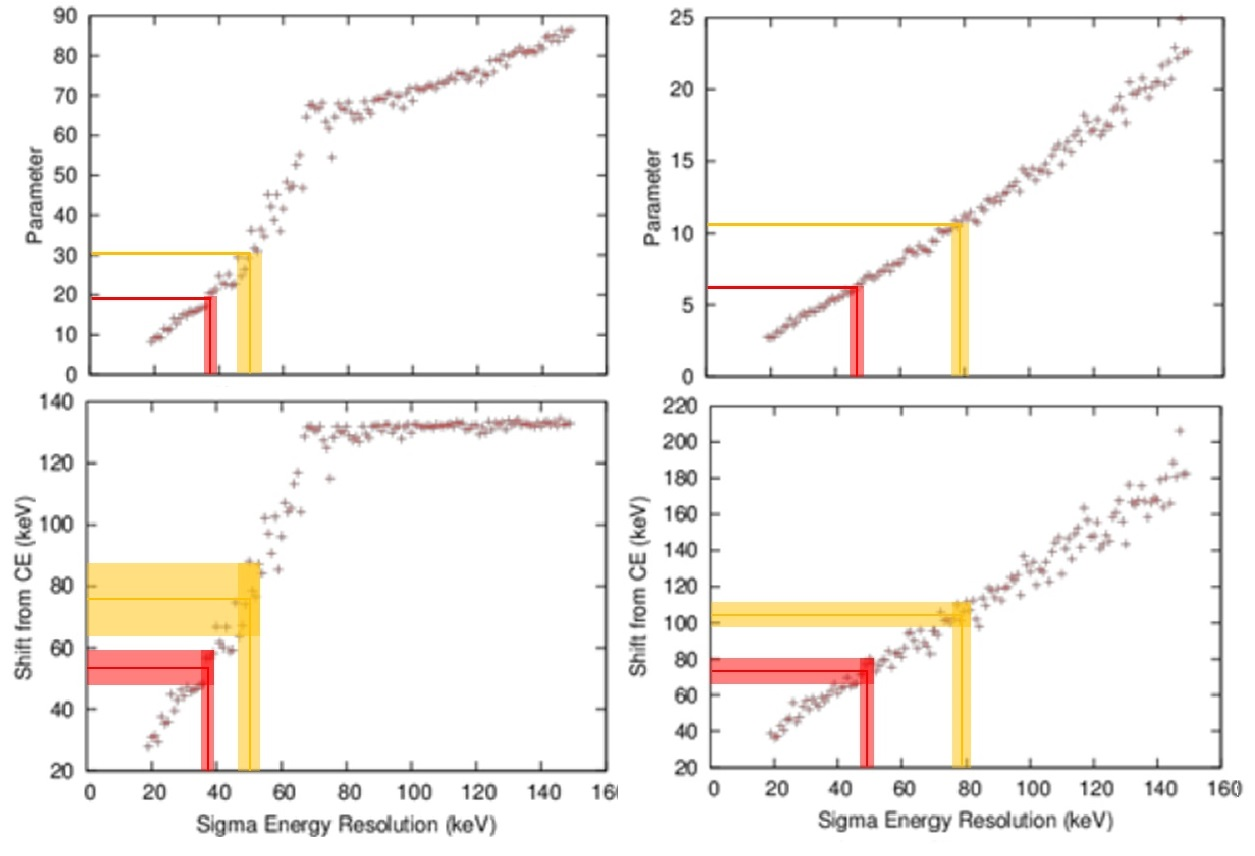
\includegraphics[scale=0.44]{en_cal_figures/Compton_shift - Copia.jpg}}
     \caption{Simulated response functions used to determine the shift from CE starting from the knowledge of parameter $\sigma/C$. Left panels: 511 keV photons; right panels: 1275 keV photons. Red lines correspond to D\#1, while orange lines correspond to D\#2.}
    \label{fig: find Compton shift}
\end{SCfigure}}

\begin{table}[t]
    \centering
    \begin{tabular}{|l|cccccccc|}
    \hline
      \multirow{2}*{Detector} & $E_\gamma$  & $E_{\mathrm{CE}}$ & $C$ &$\sigma$ &$\sigma/C$ &en. res. &$\Delta E_\mathrm{CE}$ & $E_\mathrm{CE}^{\mathrm{shifted}}$ \\
       &(keV) & (keV) & (channels) &(channels)& (\%) &(keV) &(keV) & (keV)\\
      \hline
      \multirow{2}*{D\#1}  & 511 & 341 & $834.6\pm 0.8$ & $120.8\pm 0.9$ & $19.0\pm 0.1$ & $38\pm 2$ & $53\pm 4$ & $288\pm4$\\
      & 1275& 1062& $1858.3\pm 0.7$ & $116.5\pm 0.5$ & $6.27\pm 0.03$ & $47\pm 2$ & $71\pm 4$ & $991\pm 4$\\
      \hline
       \multirow{2}*{D\#2}   & 511 & 341 & $298.8\pm 0.6$ & $90.7\pm 0.5$ & $30.3\pm 0.2$ & $50\pm 2$ & $76\pm 6$ & $265\pm 6$\\
      & 1275& 1062& $1063\pm 1$ & $114.4\pm 0.8$ & $10.77\pm 0.07$ & $78\pm 2$ & $104\pm 4$ & $958\pm 4$\\
       \hline
    \end{tabular}
    \caption{Energy of the gamma-ray ($E_\gamma$), theoretical energy of the Compton edge ($E_{\mathrm{CE}}$), parameters of the Gaussian fit performed on Fig. \ref{fig: histo calibration d1 d2} ($C$ and $\sigma$) and their ratio, values obtained from the response functions (sigma energy resolution and shift from CE $\Delta E_\mathrm{CE}$) and computed energy value of the Compton maximum ($E_\mathrm{CE}^{\mathrm{shifted}}$), both for D\#1 and D\#2}
    \label{tab: energy calibration of D1 and D2}
\end{table}
By fitting the pairs $(C, E_{\mathrm{CE}}^{\mathrm{shifted}})$ of each detector with a linear function (Fig. \ref{fig: linear fit energy calibration}), we got the parameters of the energy-channels conversion relation:
\begin{subequations}
     \begin{gather}
    \text{D\#1:}\quad  \mathrm{energy\,[keV]}=(0.687\pm0.006)\tfrac{\mathrm{keV}}{\mathrm{ch}}\cdot\mathrm{ch.\,number\,[ch]}+(-286\pm8)\,\mathrm{keV}\\
\text{D\#2:}\quad \mathrm{energy\,[keV]}=(0.91\pm0.01)\tfrac{\mathrm{keV}}{\mathrm{ch}}\cdot\mathrm{ch. \,number\,[ch]}+(-6\pm20)\,\mathrm{keV}
\end{gather}
\end{subequations}


% \begin{table}[H]
%     \centering
%     \begin{tabular}{l|cc}
%     \toprule
%     \multirow{2}*{Detector} &$a $  & $b$ \\
%     & (keV) &(keV/channels) \\
%     \hline
%    D\#1 & $-290\pm10$ & $0.69\pm0.01$ \\
%     D\#2 & $-6\pm20$ & $0.91\pm0.02$ \\
%     \bottomrule
%     \end{tabular}
%     \caption{Parameters of the linear fits in fig. \ref{fig: linear fit energy calibration}, where $y[\mathrm{keV}]=a+b\cdot x[\mathrm{channels}]$}
%     \label{tab: energy calibration parameters}
% \end{table}

\begin{figure}[H]
    \centering
    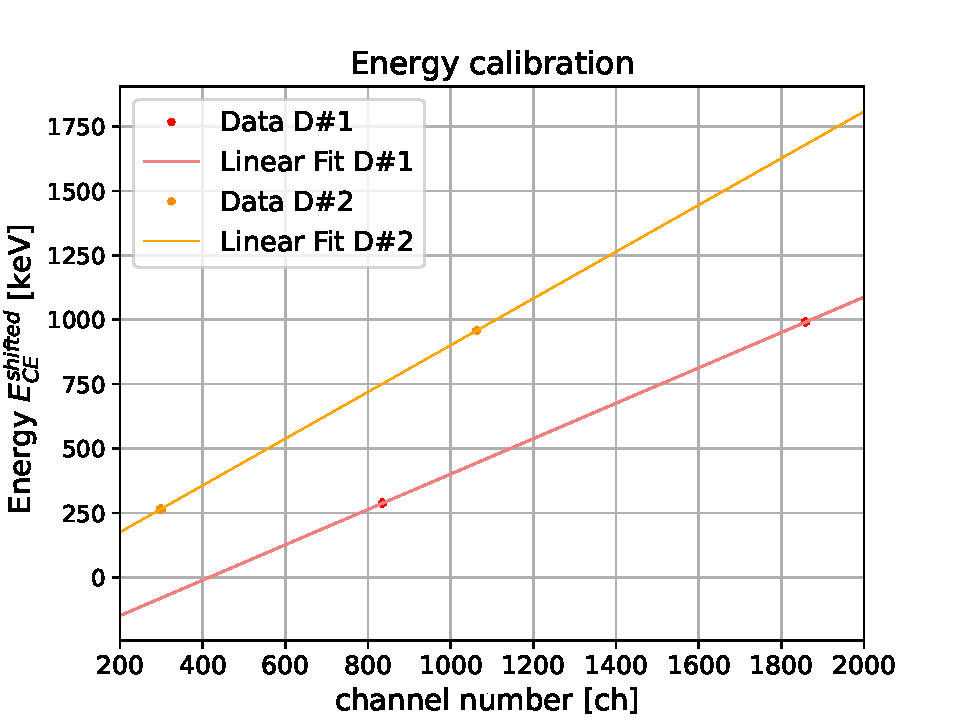
\includegraphics[width=0.48\linewidth]{en_cal_figures/energy_cal.pdf}
    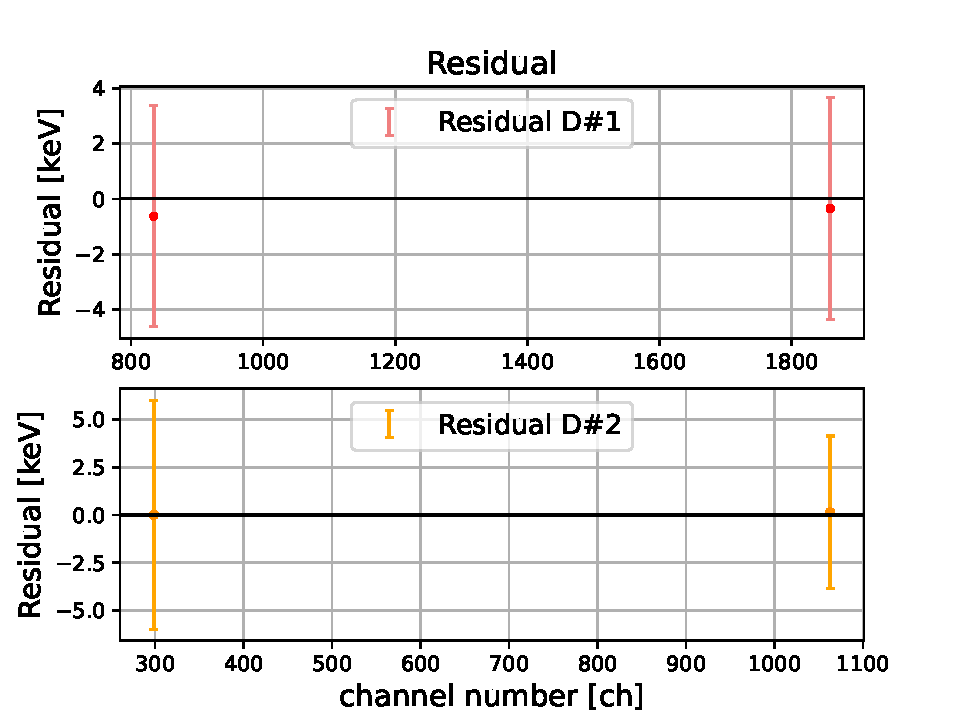
\includegraphics[width=0.48\linewidth]{en_cal_figures/res_energy_cal.pdf}
    \caption{Energy calibration of D\#1 (red) and D\#2 (orange) and residuals: on the x-axis the centroid $C$ and on the y-axis $E_{\mathrm{CE}}^{\mathrm{shifted}}$ (see Tab. \ref{tab: energy calibration of D1 and D2})}
    \label{fig: linear fit energy calibration}
\end{figure}

When looking at the calibrated spectra (Fig. \ref{fig: histo calibration d1 d2}, upper x-axis), it is apparent that in the spectrum of D\#1 there are several events corresponding to negative energies, which is unreasonable. 
Since with the available data it is not possible to find the reason nor to correct the calibration, in the following analysis, especially in Sections \hyperlink{2.3.4}{2.3.4} and \hyperlink{2.5.4}{2.5.4} dedicated to time resolution as a function of the energy, %in which the results for the energy calibration are essential, 
we will use only the calibration of D\#2.


\subsection{Analog CFDs}\label{sect: Analog CFDs}
\subsubsection{Calibration of the TAC}
\hypertarget{2.3.1}{}
In order to study the time resolution obtained with analog electronics, it is necessary, first of all, to  calibrate the TAC 
% (\textit{Time to Amplitude}) 
spectrum to obtain the results in nanoseconds. Calibration is done by correlating different time delays between the START and STOP pulses with the TAC output measured by the digitizer (CH2)\footnote{The extra delay introduced by possible differences in cable lengths is neglected.}. %TAC was connected to ch2 of the digitazer

Let us introduce seven different delays ($T_{\mathrm{delay}}\approx t_{\mathrm{stop}}-t_{\mathrm{start}}$), between $2$ and $30\,\mathrm{ns}$, in the DELAY Unit\footnote{We neglected the uncertainties of the delay values.}. For every delay, let us acquire a 10 minutes TAC spectrum\footnote{The TAC range was set at $50\,\mathrm{ns}$ multiplied by 10. Let us remember that every setting in TAC range must be divided by $\approx$10.}, in channels units, and make a Gaussian fit on the distribution. An example of the TAC spectrum and of the Gaussian fit is shown in Fig. \ref{fig: time histo} for a delay of $T_\mathrm{delay}=14\,\mathrm{ns}$, whereas the numerical results of the centroids $C$ are given in Tab. \ref{tab:TAC_cal}. 
\begin{table}[H]
\parbox{.45\linewidth}{
\centering \captionsetup{width=.7\linewidth}
 \begin{tabular}{|c|c|}
        \hline
        $T_{\mathrm{delay}}$ $\left[ \mathrm{ns}\right]$ &  $C\,\,\left[\mathrm{ch}\right]$ \\
        \hline
        2	& $	386.02	\pm	0.05    $ \\
        6	& $	514.48	\pm	0.05	$ \\
        10	& $	639.32	\pm	0.05	$ \\
        14	& $	760.26	\pm	0.06	$ \\
        18	& $	878.91	\pm	0.06	$ \\
        24	& $	1050.17	\pm	0.07	$ \\
        30	& $	1223.66	\pm	0.08	$ \\
        \hline
    \end{tabular}
    \caption{Experimental points for TAC calibration}
    \label{tab:TAC_cal}}
% \hfill
\hspace{-3.5 cm}
\parbox{.55\linewidth}{
\centering
\begin{figure}[H]
    \centering
    \captionsetup{width=.5\linewidth}
    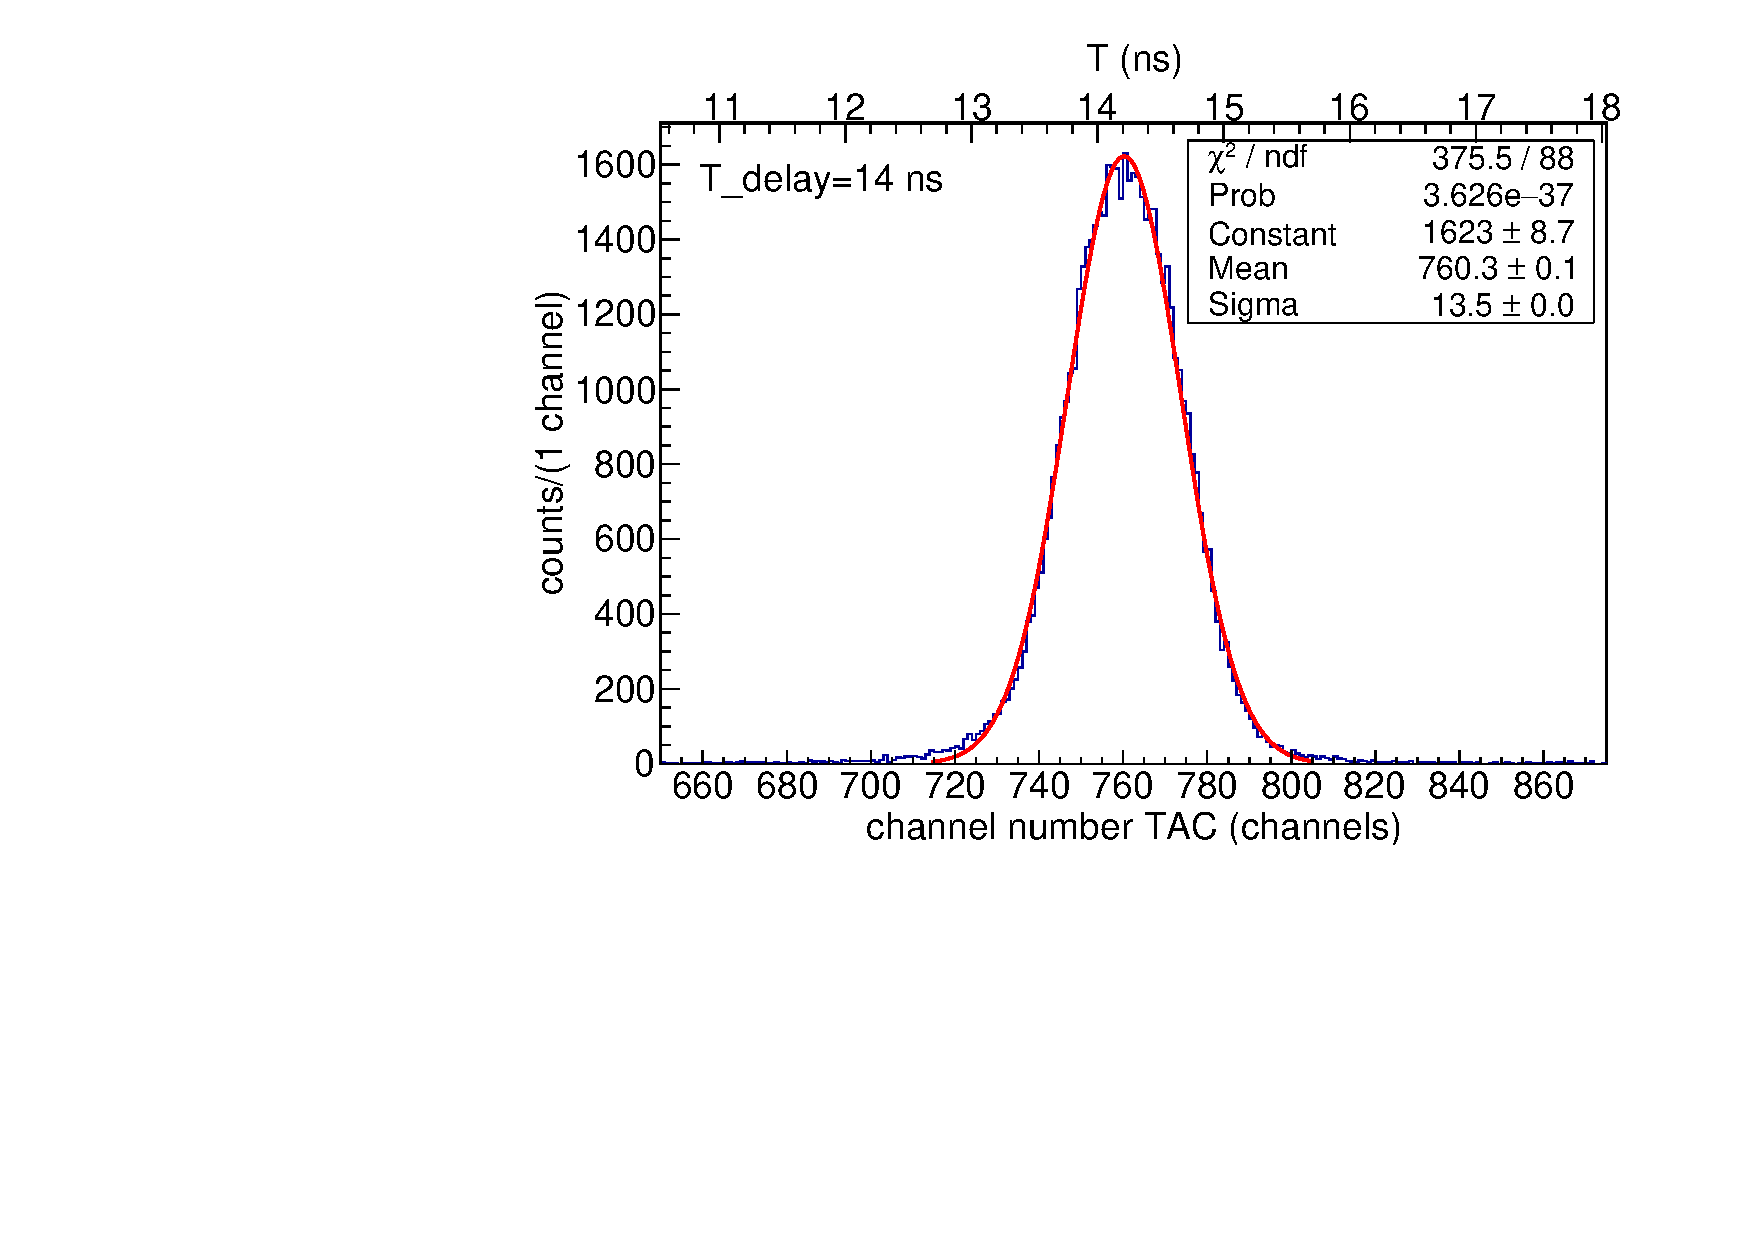
\includegraphics[width=0.5\linewidth]{tac_cal_figures/h14ns_fit_doubleAxis3.pdf}
     \caption{Time spectrum obtained with $T_\mathrm{delay}\!=\!14$ ns and Gaussian fit. On the upper x-axis it is possible to see the already calibrated spectrum.}
    \label{fig: time histo}
\end{figure}
}
\end{table}

\begin{comment}
\begin{table}[H]
    \centering
    \begin{tabular}{|c|c|}
        \hline
        delay $\left[ \mathrm{ns}\right]$ &  $C\,\,\left[\mathrm{ch}\right]$ \\
        \hline
        2	& $	386.02	\pm	0.05    $ \\
        6	& $	514.48	\pm	0.05	$ \\
        10	& $	639.32	\pm	0.05	$ \\
        14	& $	760.26	\pm	0.06	$ \\
        18	& $	878.91	\pm	0.06	$ \\
        24	& $	1050.17	\pm	0.07	$ \\
        30	& $	1223.66	\pm	0.08	$ \\
        \hline
    \end{tabular}
    \caption{TAC calibration}
    \label{tab:TAC_cal}
\end{table}
\end{comment}
Then, these data are used to obtain a linear fit, with delays in $\mathrm{ns}$ on x-axis and the centroids on the y-axis, according to the formula%\footnote{We evaluted that the uncertaintes on the delay of the DELAY Unit are neglectables, since they are related to the instrumentation, then we decided to put the delays in $\mathrm{ns}$ on the x-axis and the centroids on the y-axis, and then to invert the formula and propagate the uncertaintes..}
\begin{equation}\label{eq: measured time}
   C\,[ch]=m\cdot T_{\mathrm{delay}}\,[ns]+q
\end{equation}
The graph of the linear fit and the residual plot are shown in Fig. \ref{fig:TAC_cal}: from the residual graph it is possible to notice that the points for lower (less than $\approx\!\!10\,\mathrm{ns}$) and higher (more than $\approx\!\!20\,\mathrm{ns}$) delays are placed below the linear fit, that is the linearity seems to be affected by a systematic curvature. Despite this observation, it is still possible to consider the points to be linear, so as to consider valid the TAC calibration results. The parameters of the linear fit and the respective relative errors are
\begin{table}[H]
    \centering
    \begin{tabular}{c|c}
    \hline
    $m=(30.0\pm0.3) \, \frac{\mathrm{ch}}{\mathrm{ns}}$ & $0.010$\\
    $q=(334\pm5) \,\mathrm{ch}$ & $0.015$\\
    \hline
    \end{tabular}
    \caption{Results of TAC calibration and relative errors}
    \label{tab:TAC_cal_results}
\end{table}
%29.99819555, 333.94321446
%0.317536835432671
%4.674924198585312

\begin{figure}[H]
    \centering
    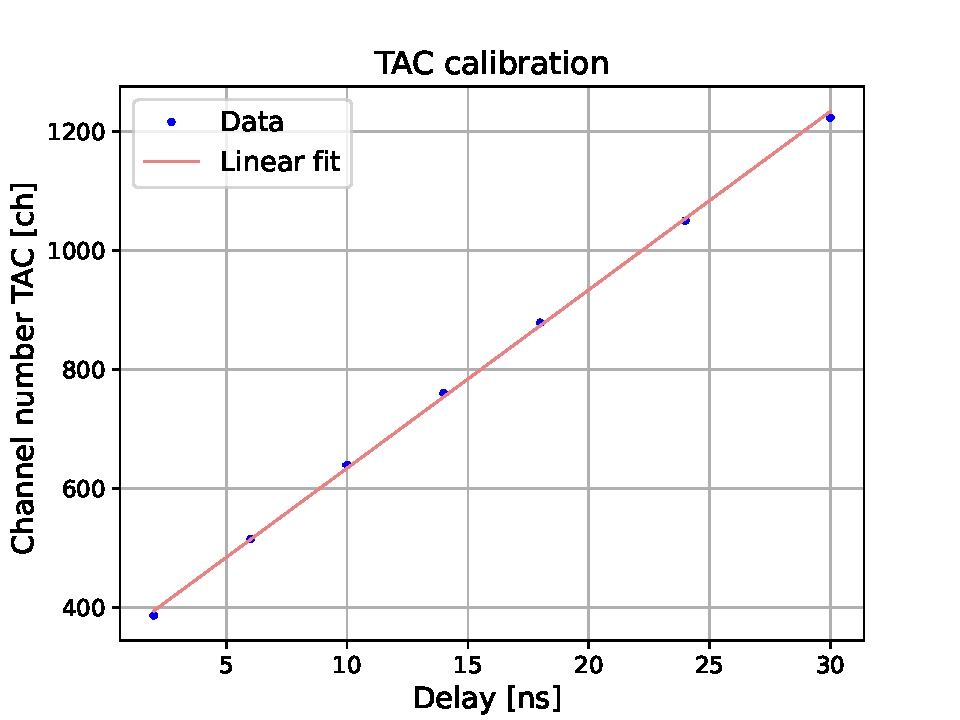
\includegraphics[width=0.5\linewidth]{tac_cal_figures/Tac_cal.pdf}
    \hspace{-0.6 cm}
    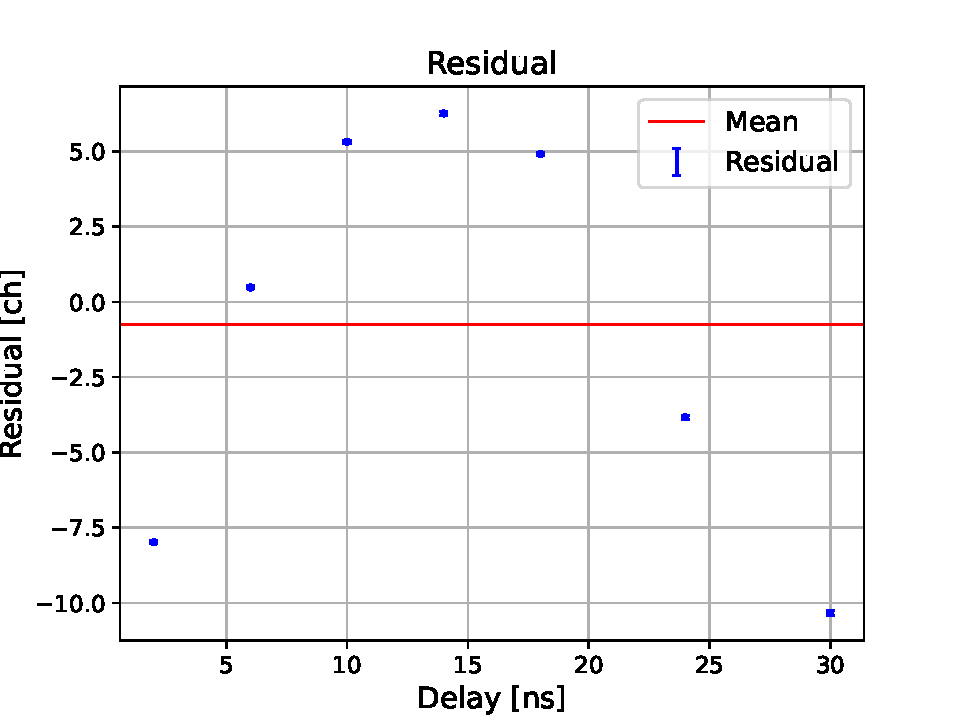
\includegraphics[width=0.5\linewidth]{tac_cal_figures/res_tac_cal.pdf}
    \caption{TAC calibration and residuals (see Tab. \ref{tab:TAC_cal})}
    \label{fig:TAC_cal}
\end{figure}

\subsubsection{Calibration of the delay cable}
\hypertarget{2.3.2}{}

This paragraph is dedicated to the study of the delay $t_c$ introduced by variable lengths of LEMO cables, which will be used next as external delays in the CFDs. Now the delay of the DELAY Unit $t_D$ is set to $8\,\mathrm{ns}$ and this will be kept until the end of Section \ref{sect: Analog CFDs}.
%in the next measurements. 
With the addition of a LEMO cable before the STOP of the TAC, the final delay $T_{\mathrm{delay}}$ increases of a quantity $t_c$:
$$T_{\mathrm{delay}}=t_D+t_c$$

Because the fraction of the CFDs is fixed at 20\%, the required cable should introduce a delay of about the $80\%$ of the downfall time measured previously, i.e. between $4.7\,\mathrm{ns}$ and $5.5\,\mathrm{ns}$ considering both detectors. 
Let us consider two different cables of about $45\,\mathrm{cm}$ and $90\,\mathrm{cm}$. In particular, the first one was made of two short cables, whereas the second one was given by four short cables: each short LEMO cable, which is expected to introduce a delay of about $1\,\mathrm{ns}$, 
% \textcolor{red}{(\textit{this is going to be tested in this section})}
is about $(21.5\pm0.3)\,\mathrm{cm}$ long and let us consider about $1\,\mathrm{cm}$ for every connection between two short cables. 
Due to the availability of cables and to the big uncertainties associated to the ruler used for measure and especially considering the aim of this study, in this report there are not any precise measurements of the lengths of the cables and it is preferred to associate just a nominal length to them.

%About the length of the cables: in order to conduct the experiment properly, it was necessary to have many different cables and, iin particular, two cables of the same length for both part of the CFD, connected to D1 and D2. Then, due to the lack of time, it was not possible to measure every single cable used for the experiment. Therefore, the attention was focused just on finding the cable with the right delay and then try to used a cable of the same lenght, according to the availability of the cables in the laboratory and of the measurements necessary on the next steps of the experiment.
%Furthermore, due to the last consideration, we prefer not to make a linear fit with just two point and any good measure of length.

For each compound cable, a 10 minutes TAC spectrum was acquired and a Gaussian fit was made as in the previous \hyperlink{2.3.1}{paragraph}. Finally, by using the parameters $m$ and $q$ of TAC calibration and by subtracting the delay of the DELAY Unit $t_D$, it is possible to convert the resulting centroids $C$ in nanoseconds, so as to obtain the delay $t_c$ introduced by each cable expressed in ns:
\begin{equation}\label{eq:conversion}
    t_c=\dfrac{C-q}{m}-t_D
\end{equation}
% where $m$ and $q$ the parameters of the linear fit.
% Since the uncertainties on the centroids of the fits look underestimated, 
Let us consider also the errors on the parameters of the fit and propagate the errors. %we don't have to say so necessarily
The numerical results %for cable calibration 
are shown in the Tab. \ref{tab:cable_cal}, %in the first column the cable length $L$, as discussed before, 
where $L$ is the LEMO cable length, as discussed before.
% in the middle one the centroids $C$ and in the column on the right the delay introduced by each cable converted in ns, according to the formula \ref{eq:conversion}. 

\begin{table}[H]
    \centering \captionsetup{width=.55\linewidth}
    \begin{tabular}{|c|cc|}
    \hline
    $L\,\left[\mathrm{cm}\right]$ & $C\,\left[\mathrm{ch}\right]$ & $t_c\,\left[\mathrm{ns}\right]$ \\
    \hline
    $45$ & $639.17\pm0.07$ & $2.2\pm0.2$ \\ 
    $90$ & $708.57\pm0.07$ & $4.5\pm0.2$\\ 
    \hline
    \end{tabular}
    \caption{Centroid $C$ of TAC output and delay $t_c$ introduced by a cable of length $L$}
    \label{tab:cable_cal}
\end{table}

Assuming a linear relation between the length and the delay, and %so with 
performing a linear fit, 
it would be possible to 
%obtain a calibration as in the previous paragraph, then to 
estimate the delay introduced by any cable just by knowing its length. However, since the measure of the length is not accurate and it was possible to measure just two series of cables, it is preferable not to do a linear fit. The expected delay $t_c$ for a given LEMO cable can still be roughly estimated from the acquired two points, by noticing that the delay is about 5 ns/m.


\subsubsection{Time resolution as a function of the external delay of the CFDs}
The following two sections deal with the study of the time resolution as a function of the external delay of the CFDs and, secondly, as a function of the energy (Section \hyperlink{2.3.4}{2.3.4}). Let us begin with the external delay $D$: as mentioned in the previous paragraph, the expectation is to find the best time resolution when the external delay is the $80\%$ of the falling time of the signal.

The external delay was realized by using a LEMO cable for each detector. Considering the results of the previous paragraph (with $t_c\equiv D$), it is possible to assume that cables of about $100\, \mathrm{cm}$ will imply the smallest time resolution\footnote{As explained in previous section, the precision of the measurement was strongly constrained by the availability of cables.}. 
Then, three different cables were used for the experiment: the main one is about $100\,\mathrm{cm}$ long, then a shorter cable and a longer one were used in order to verify the minimum around the expected value. The next table (Tab. \ref{tab:time_res_delay}) lists the values of the lengths $L$ of the cables and the associated FWHMs of TAC output (in channels), calculated as $\mathrm{FWHM}=2.35\sigma$, where $\sigma$ is the standard deviation of the Gaussian. In this analysis, the FWHM corresponds to the time resolution $R=\tfrac{\mathrm{FWHM}}{m}$ (in the third column in $\mathrm{ns}$)\footnote{The uncertainties on the resolution values consider the errors on the parameter $m$ of the TAC calibration.}. %to not underestimate them
%asymmetry on the gaussian fit
The same results are shown in the Fig. \ref{fig:time_res_delay}, where on the x-axis there is the cable length, whereas on y-axis the time resolution. The plot displays a minimum around the expected value discussed before, but, %as for the cable calibration, 
being the points too few, it is preferable not to make any parabolic fit to show approximately where the minimum is.

\begin{table}[H]
\parbox{.45\linewidth}{
 \centering
 % \captionsetup{width=.5\linewidth}
 \begin{tabular}{|c|cc|}
    \hline
    $L \,\left[\mathrm{cm}\right]$& FWHM $\left[\mathrm{ch}\right]$ &$R\,\left[\mathrm{ns}\right]$\\
    \hline
    $60$ & $40.68\pm0.09$ & $1.36\pm0.01$ \\
    $100$ & $31.47\pm0.07$ & $1.05\pm0.01$ \\
    $120$  & $35.34\pm0.09$ & $1.18\pm0.01$ \\
    \hline
    %\bottomrule
    \end{tabular}
    \caption{FWHM and time resolution $R$ as a function of the external delay %$t_c$ 
    introduced by cables of length $L$}
    \label{tab:time_res_delay}}
% \hfill
 \hspace{-3 cm}
\parbox{.55\linewidth}{
\centering
\begin{figure}[H]
    \centering
    \captionsetup{width=.45\linewidth}   
    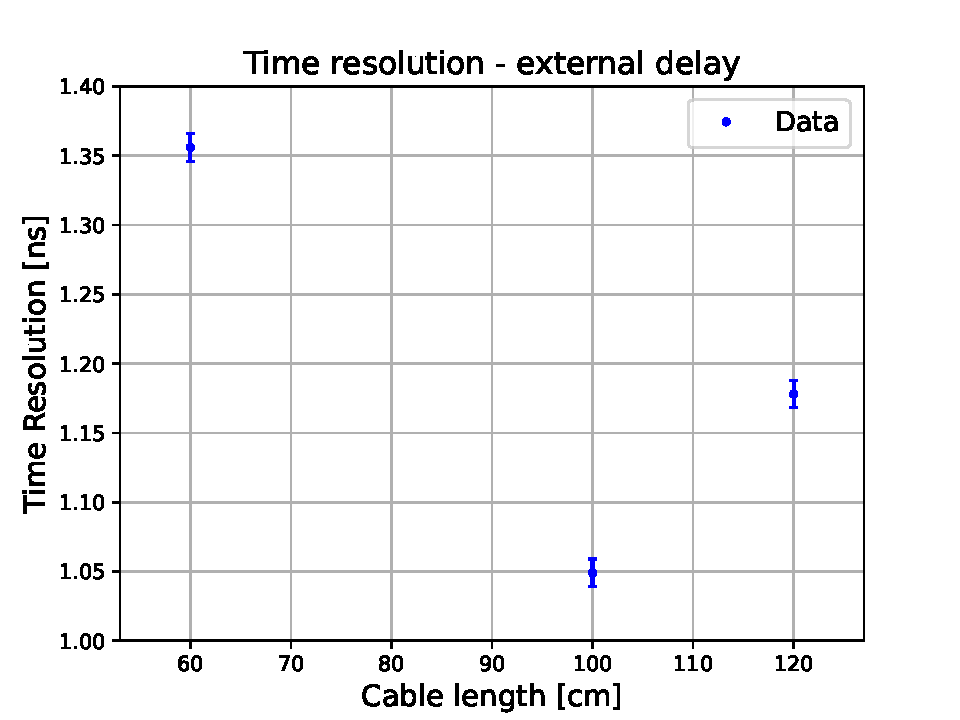
\includegraphics[width=0.5\linewidth]{res_vs_energy_figures/time_res_delay.pdf}
    \caption{Time resolution as a function of length of the cable providing the external delay (see Tab. \ref{tab:time_res_delay})}
    \label{fig:time_res_delay}
\end{figure}
}
\end{table}

% \begin{table}[H]
%     \centering \captionsetup{width=.55\linewidth}
%     \begin{tabular}{|c|cc|}
%     \hline
%     $L \,\left[\mathrm{cm}\right]$& FWHM $\left[\mathrm{ch}\right]$ &$R\,\left[\mathrm{ns}\right]$\\
%     \hline
%     $60$ & $40.68\pm0.09$ & $1.36\pm0.01$ \\
%     $100$ & $31.47\pm0.07$ & $1.05\pm0.01$ \\
%     $120$  & $35.34\pm0.09$ & $1.18\pm0.01$ \\
%     \hline
%     %\bottomrule
%     \end{tabular}
%     \caption{FWHM and time resolution $R$ as a function of the external delay %$t_c$ 
%     introduced by cables of length $L$}
%     \label{tab:time_res_delay}
% \end{table}

% \begin{figure}[H]
%     \centering
%     \captionsetup{width=.65\linewidth}   
%     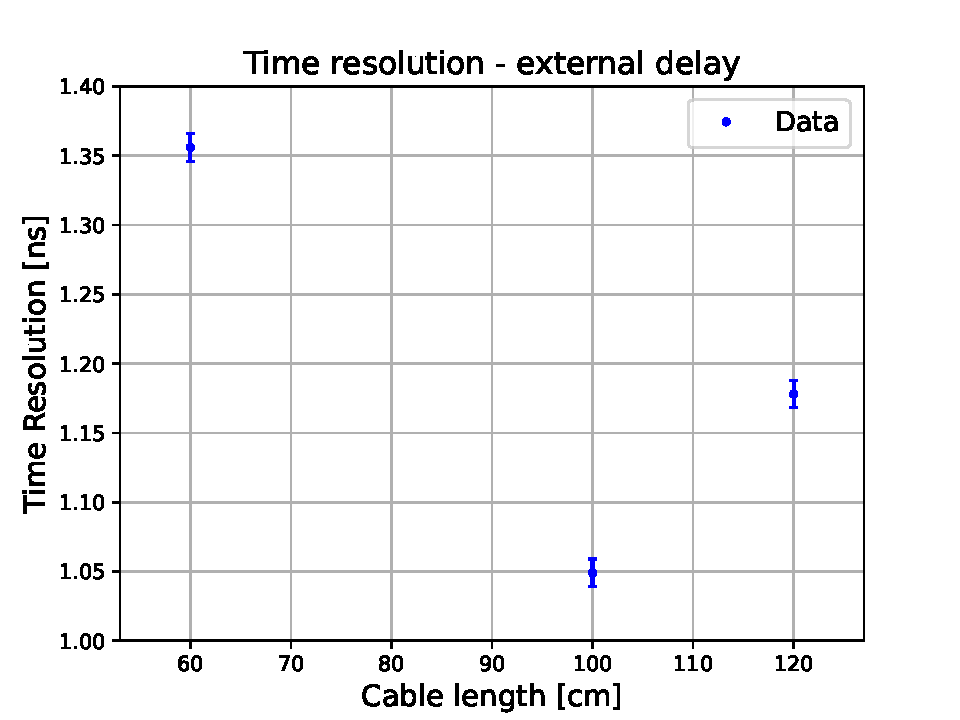
\includegraphics[width=0.5\linewidth]{res_vs_energy_figures/time_res_delay.pdf}
%     \caption{Time resolution as a function of length of the cable providing the external delay (see Tab. \ref{tab:time_res_delay})}
%     \label{fig:time_res_delay}
% \end{figure}

%other discussion of the results

\subsubsection{Time resolution as a function of the energy range}
\hypertarget{2.3.4}{}
In this paragraph, the relationship between the resolution of the timing measurement and the energy of the recorded events is studied. 
The \ce{^{22}Na} source was replaced with a \ce{^{60}Co} source, which has two coincident
gamma-rays at 1173 and 1332 keV. 
The energy and time spectra of the source were recorded over a period of roughly 20 hours. 
The delay before the STOP of the TAC was set again at 8 ns.

As for the energy spectrum, let us consider only the one acquired by D\#2, since its calibration turned out to be more reliable with respect to that of D\#1 (Section \ref{sect: energy calibration}). 
Figure \ref{fig: 2D histo res vs energy} shows the correlation between the calibrated energy spectrum of D\#2 and the calibrated time spectrum recorded on CH2. 
As expected, the former displays a Compton continuum ending at about 1 MeV. 
The latter consists of a peak whose position first decreases with energy, then remains approximately constant. 
Besides, its tails are not symmetric: for a given energy window, there are more events accumulating on the left of the peak (lower time differences) than on the right (higher time differences).
% This may be due either to a systematic overestimate of $t_1$ or to a systematic underestimate of $t_2$ for some events (see Eq. \eqref{eq: measured time}).
% \textcolor{blue}{EXPLANATIONS + OTHER POSSIBLE CAUSES}
Since the output of the TAC can be described as $t_{D\#2}-t_{D\#1}+T_{\mathrm{delay}}$, an higher position of the TAC peak for lower energies of signals recorded by D\#2 may be caused by an overestimate of $t_{D\#2}$ for low signals. 
This means that at least the CFD associated to D\#2 is not working very well, maybe because of the non optimal value of the WALK ADJ.

%baseline messa male o  troppa dispersione -> cfd non funziona bene

%errore nell'ottimizzazione del segnale


\begin{figure} [H]
    \centering %\captionsetup{width=.71\linewidth}
    %\captionsetup{width=.65\linewidth}
    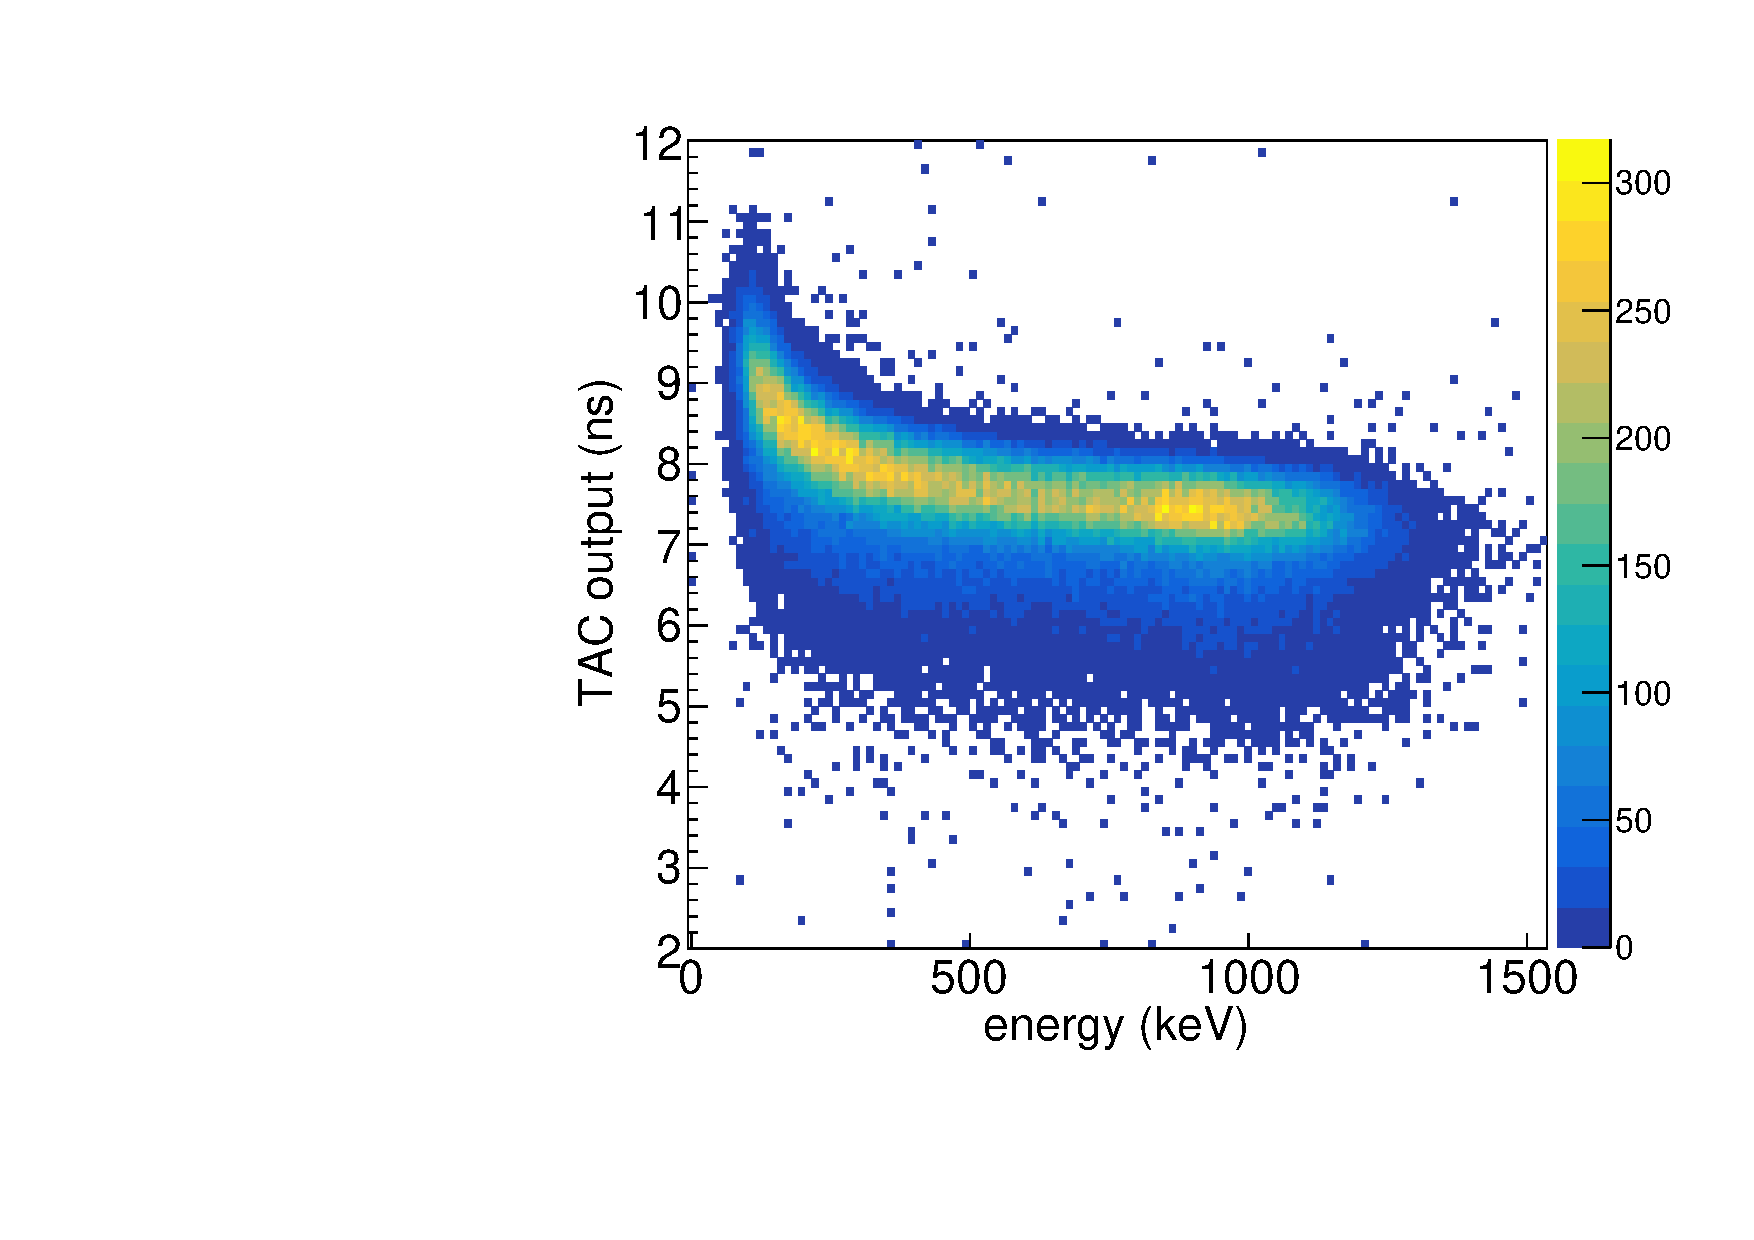
\includegraphics[scale=0.38]{res_vs_energy_figures/2D_histo_en,time_calibrated2.pdf}
    
    \caption{Correlation between the energy spectrum obtained from the FPGA for D\#2 ($x$) and the coincidence time spectrum from TAC output ($y$) of the \ce{^{60}Co} source. Both axes are calibrated according to the relations previously found.}
   \label{fig: 2D histo res vs energy}
\end{figure}

Let us perform a Gaussian fit on the right side of the time peak selecting only events with energy higher than several values of a lower threshold. 
The chosen thresholds are reported in Tab. \ref{tab:res vs energy threshold}, with the FWHM of the interpolating Gaussian and its conversion in ns (time resolution $R$). 
The values of $R$ are plotted in Fig. \ref{fig:time_res_energy} as a function of the lower energy threshold.
Then the same procedure was applied to measure the resolution when considering only events whose energy belongs to a certain window, i.e. also introducing an upper energy threshold. 
The results are shown in Tab. \ref{tab:res vs energy range} and in Fig. \ref{fig:time_res_energy}. In both graphics the time resolution decreases as a function of the energy and, in particular, let us notice that for the graphic on the left this value seems to increase again for the last two points (i.e. for a lower energy threshold at $950$ and $1000\, \mathrm{keV}$).

\begin{table}[H]
\parbox{.45\linewidth}{
\centering
\begin{tabular}{|c|cc|}
  \hline
       lower en. th.  &  FWHM  & $R$ \\
       (keV) & (channels) & (ns)\\
      \hline
        $100$ & $33.2\pm 0.1$ & $1.11\pm0.01$\\
      $150$ & $32.9\pm0.1$ & $1.10\pm0.01$\\
      $200$  & $32.3\pm0.1$ & $1.08\pm0.01$\\
      $250$  & $30.13\pm0.08$ & $1.00\pm0.01$\\
      $300$  & $28.04\pm0.07$ & $0.93\pm$0.01\\
      $350$  & $26.53\pm0.07$ & $0.88\pm$0.01\\
      $400$  & $25.27\pm0.07$ & $0.842\pm0.009$\\
      $450$  & $24.25\pm0.07$ & $0.808\pm0.009$\\
      $500$  & $23.48\pm0.07$ & $0.783\pm0.009$\\
      $550$  & $22.80\pm0.07$ & $0.760\pm0.008$\\
      $600$  & $22.49\pm0.07$ & $0.750\pm0.008$\\
      $650$  & $22.30\pm0.08$ & $0.743\pm0.008$\\
      $700$  & $22.04\pm0.07$ & $0.735\pm0.008$\\
      $750$  & $21.92\pm0.08$ & $0.731\pm0.008$\\
      $800$  & $22.18\pm0.08$ & $0.739\pm0.008$\\
      $850$  & $22.09\pm0.09$ & $0.736\pm0.008$\\
      $900$  & $21.9\pm0.1$ & $0.731\pm0.008$\\
      $950$  & $22.2\pm0.1$ & $0.739\pm0.009$\\
      $1000$  & $22.3\pm0.1$ & $0.743\pm0.009$\\
     
         \hline
\end{tabular}
\caption{FWHM and time resolution $R$ as a function of the lower energy threshold}\label{tab:res vs energy threshold}
}
\hfill
\parbox{.45\linewidth}{
\centering
\begin{tabular}{|c|cc|}
  \hline
       en. range  &  FWHM  & $R$ \\
       (keV) & (channels) & (ns)\\
      \hline
        $[50;150]$ & $39.7\pm0.4$ & $1.32\pm0.02$\\
          $[150;250]$ & $32.3\pm0.2$ & $1.08\pm0.01$\\
      $[250;350]$ & $26.4\pm0.2$ & $0.88\pm0.01$\\
        $[350;450]$ & $24.1\pm0.2$ & $0.80\pm0.01$\\
      $[450;550]$ & $23.0\pm0.2$ & $0.77\pm0.01$\\
        $[550;650]$ & $22.4\pm0.2$ & $0.75\pm0.01$\\
      $[650;750]$  & $22.1\pm0.2$ & $0.74\pm0.01$\\
        $[750;850]$ & $21.5\pm0.1$ & $0.72\pm0.01$\\
      $[850;950] $ & $20.7\pm0.1$ & $0.69\pm0.01$\\
         \hline
\end{tabular}
\caption{FWHM and time resolution $R$ as a function of the energy range}\label{tab:res vs energy range}
}
\end{table}

\begin{figure}[H]
    \centering
    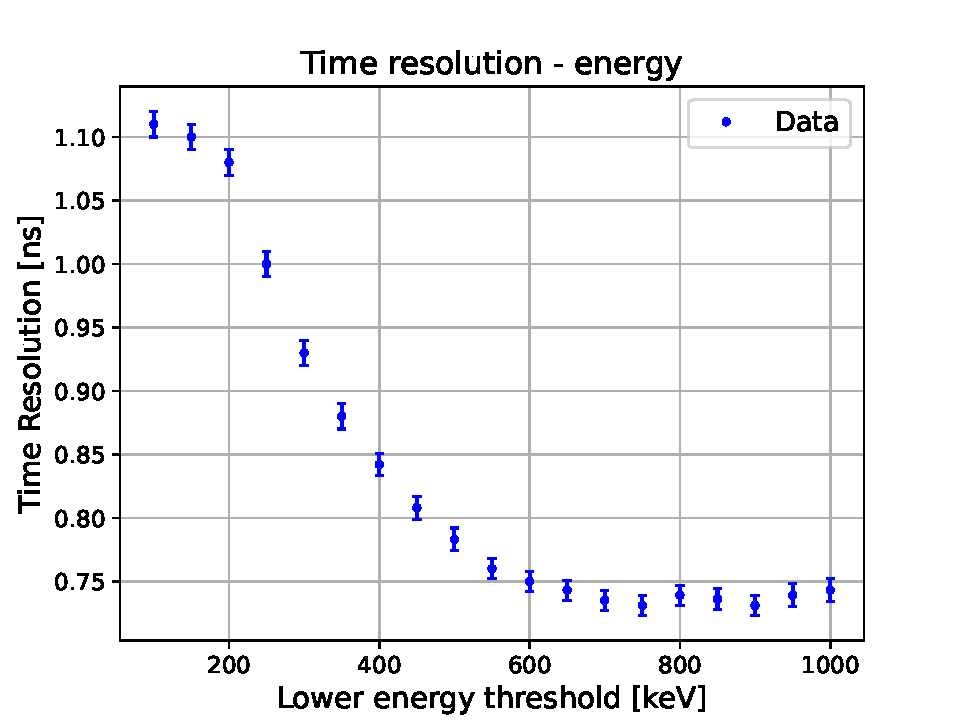
\includegraphics[width=0.51\linewidth]{res_vs_energy_figures/time_res_energy.pdf}
    \hspace{-0.8 cm}
    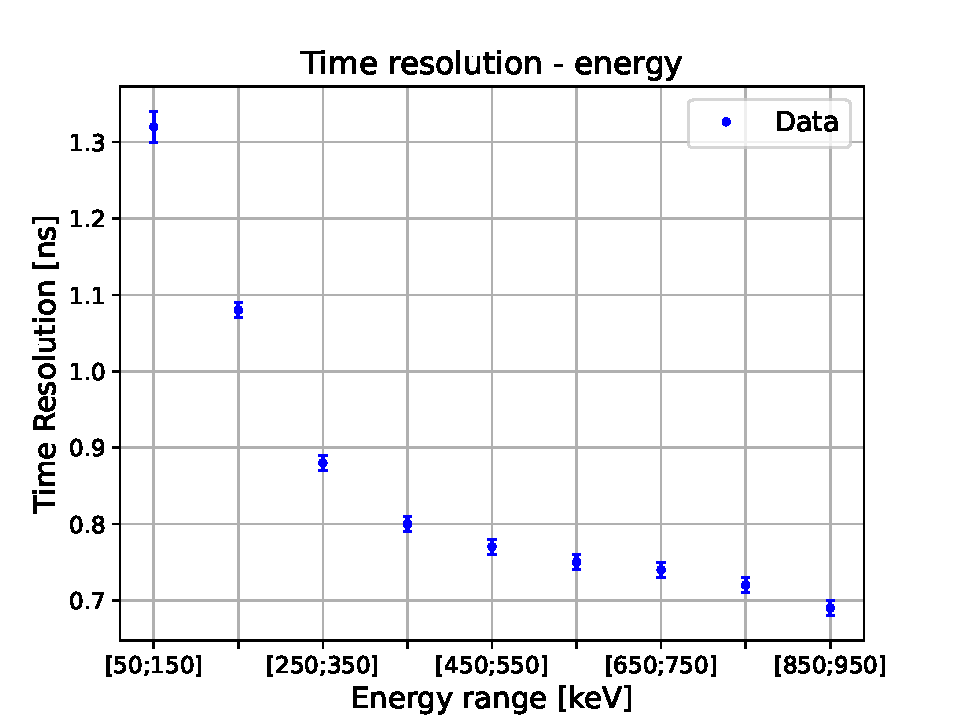
\includegraphics[width=0.51\linewidth]{res_vs_energy_figures/time_res_energy2.pdf}
    \caption{Left panel: time resolution as a function of the lower energy threshold (see Tab. \ref{tab:res vs energy threshold}); right panel: time resolution as a function of the energy range (see Tab. \ref{tab:res vs energy range})}
    \label{fig:time_res_energy}
\end{figure}



\subsection{Measurement of the speed of light}
\hypertarget{2.4}{}
The detectors were slid to one end of the guide each. 
Two 45 minutes time spectra were acquired, differing in the position of the \ce{^{22}Na} source between the detectors: in configuration 1 the source distance from D\#2 was $x_1$, in configuration 2 it was $x_2<x_1$. 
Because the source is not equidistant from the detectors, the two coincidence photons do not have the same time of arrival to the respective detectors. 
The output of the TAC will be sensitive to that time difference ($t_{\mathrm{D\#2}}-t_{\mathrm{D\#1}}$); let us call it $T_1$ and $T_2$ for configurations 1 and 2 respectively. 
The speed of light can be estimated through the relation%as well as to the fixed delay time $T_{\mathrm{delay}}$, which was set at 32 ns. 
\begin{equation}\label{eq: speed of light}
    c=\frac{2(x_1-x_2)}{T_1-T_2}=\frac{2m(x_1-x_2)}{C_1-C_2}
\end{equation}
In the last step the centroids $C_1$ and $C_2$ of the Gaussian fits were introduced, in addition to the parameter $m$ of TAC calibration\footnote{The contribution of $T_{\mathrm{delay}}$, which was set at 32 ns, simplifies.}. 

Since only the difference between $x_1$ and $x_2$ is involved in the formula, it is not important which part of D\#2 is chosen as the origin, provided that it is the same for both configurations. 
As for the position of the source, it was chosen as the midpoint of the lead brick. Because the point for the reading of the ruler used to measure the distances was ambiguous, let us associate to the distances $x_1,\,x_2$ a maximum dispersion of 5 mm each, with the assumption of a uniform distribution in that interval. 
The resulting estimates are given in Tab. \ref{tab: speed of light} for both configurations, together with the centroids $C$ and the corresponding differences $T$ in time of arrival.
\begin{table}[H]
    \centering \captionsetup{width=.70\linewidth}
    \begin{tabular}{|c|ccc|}
    \hline
  Configuration \#& $x$ (cm) & $C $ (ch)  & $T$ (ns)\\
    \hline
    1&  $78.0\pm0.1$ &   $1314.6\pm0.3$& $0.7\pm0.3$ \\
    2& $20.0\pm0.1$ & $1190.5\pm0.3$  & $-3.4\pm0.3$ \\
    \hline
    \end{tabular}
    \caption{Distance of the source from D\#2 ($x$), centroid of TAC output ($C$) and time difference ($t_{\mathrm{D\#2}}-t_{\mathrm{D\#1}}$) for configurations 1 and 2}
    \label{tab: speed of light}
\end{table}
The obtained estimate for the speed of light is
\[c=(2.80\pm0.03)\cdot10^8\;\mathrm{m/s}\]
where the uncertainty was calculated by propagating the errors of all the variables appearing in the last part of Eq. \eqref{eq: speed of light}. 
This estimate is not compatible with the reference value inside $6\sigma$, being underestimated by $\approx7\%$, hence a systematic error is involved. 
% This method allows us to get rid of the systematic error due
Thanks to the adopted procedure for measuring $c$, the systematic error introduced by the propagation of the photons inside the detectors should not be relevant. 
An underestimate of the distance $x_1-x_2$ is possible, but it cannot be the only cause, since otherwise a quantity as big as 4 cm would be missing.
Finally, an underestimate of the slope $m$ of TAC calibration must be taken into account.


\subsection{Digital CFDs} 
In this section, the aim of the study is to discuss the 
timing measurements and the time resolution from the digitized waveforms of the signals recorded by the digitizer and reproducing offline a digital CFD. This will be done by properly analysing and modifying the signal with a ROOT macro. Finally, the results will be compared to the ones obtained for the analogue CFDs, in the section dedicated to conclusions (Sec. \hyperlink{3}{3}).

For this acquisition, the TAC was disconnected from the digitizer and the source and the detectors were put again in the original configuration. %, so the detectors were again close to the source. 
D\#1 and D\#2 were still connected to CH0 and CH1 of the digitizer, respectively. Then, 45 minutes of in coincidence events from \ce{^{22}Na} were acquired.
\begin{figure}[H]
    \centering
    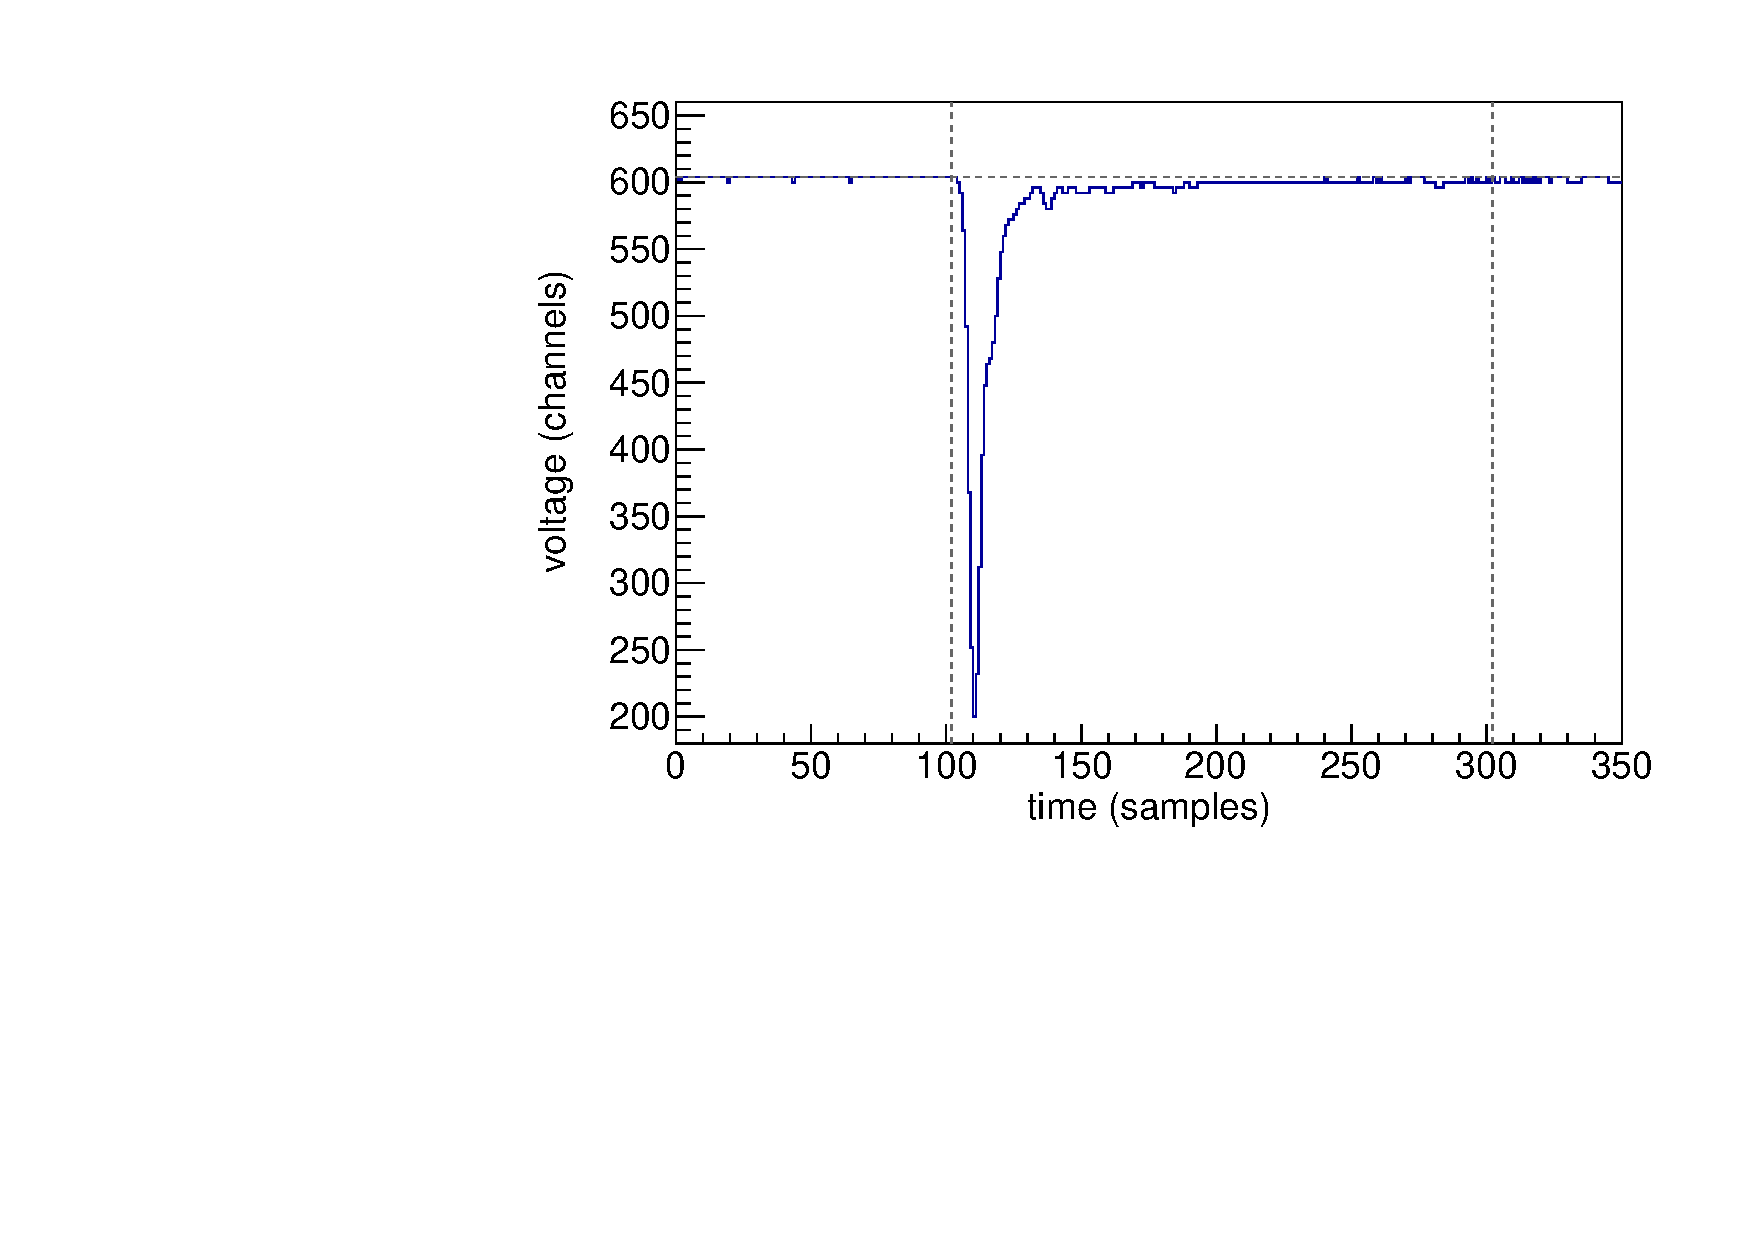
\includegraphics[width=0.48\linewidth]{digital_figures/signal7_D1_lines.pdf}
    \hspace{-0.3 cm}
    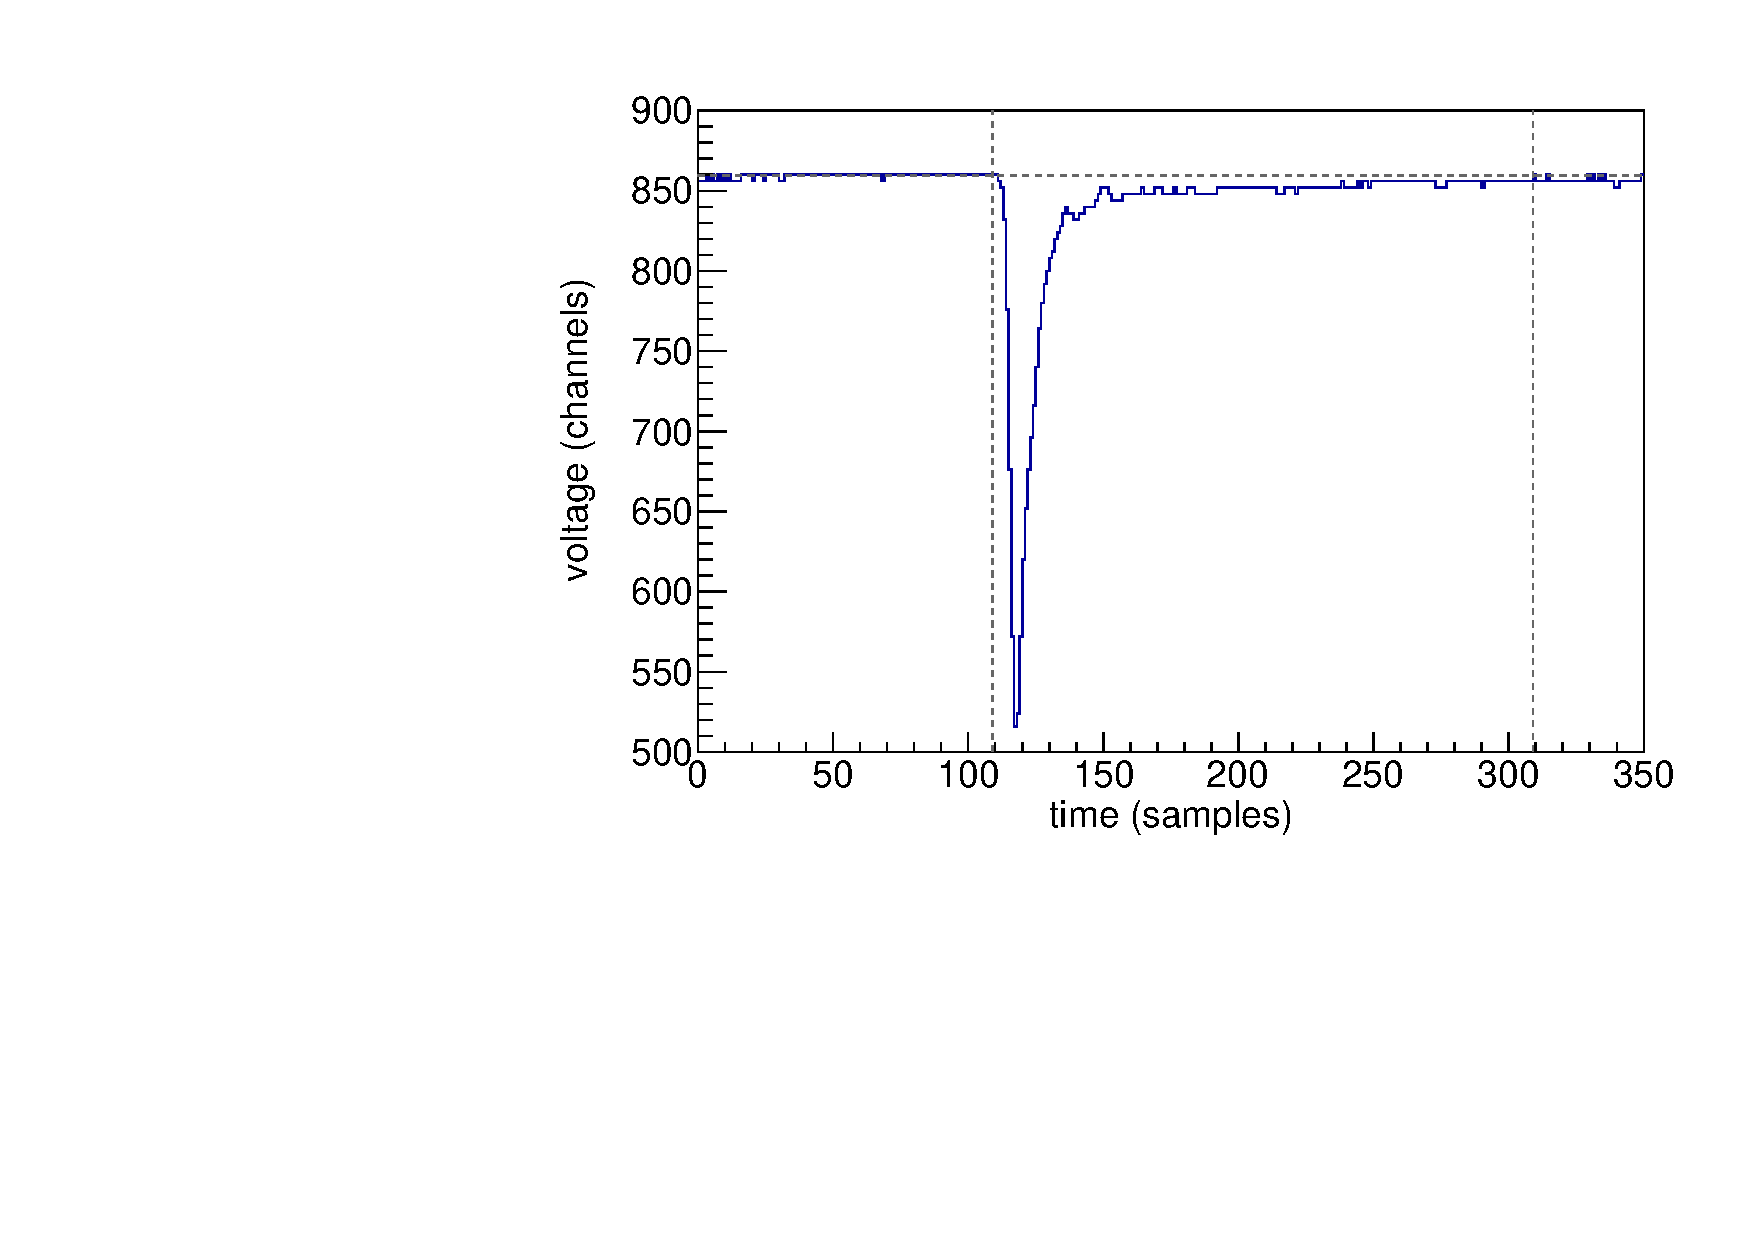
\includegraphics[width=0.48\linewidth]{digital_figures/signal7_D2_lines2.pdf}
    \caption{Waveforms of the same coincidence event as recorded by D\#1 (left) and D\#2 (right). The horizontal dashed line is the baseline estimation, while the two vertical lines are the chosen extremes for the integration.}
   \label{fig: waveform}
\end{figure}
Fig. \ref{fig: waveform} shows an example pair of waveforms acquired for the same coincident event, one by D\#1 and the other by D\#2. The sampling features of the digitizer are such that $1 \, \mathrm{sample}\!\!=\!\!
1 \,\mathrm{ns}$ and $1\,\text{ADC channel}\!\approx\!\!1\,\mathrm{mV}$. 
When considering all the events, one can see that all the pulses in the same channel have roughly the same baseline (around 600 mV for D\#1 and around 850 mV for D\#2), but their heights vary from nearly zero to the maximum value allowed by the acceptance of the digitizer (1 V). Indeed, for D\#1, several signals are more than 600 mV high, thus they result saturated. Those events are excluded from the following analysis.

Before creating the digital CFDs, the baseline and the extremes for the integration were estimated for each event in both detectors. 
By interpolating between the samples nearest to the point in which the leading edge crosses a programmable threshold, the "trigger" time is estimated. The first integration extreme is defined as the "trigger" time minus a Pre-Gate, while the second one is simply the first extreme plus a fixed Gate. 
The baseline is evaluated as the mean value of the samples between 0 and the first integration extreme. 
Because the digitizer QCD setting were not saved, the values of the threshold (550 mV for D\#1 and 830 mV for D\#2), of the Pre-Gate (4 ns) and of the Gate (200 ns) were chosen by us. 
In Fig. \ref{fig: waveform}, the baseline and the integration extremes obtained for the example waveforms are represented as straight lines.
% A threshold is defined (550 mV for D\#1 and 830 mV for D\#2). By interpolating between the samples nearest to the crossing point in the leading edge, the "trigger" time is estimated. 
% A value of 4 ns is chosen for the Pre-Gate, so that the first integration extreme is found

% The baseline, shown by the horizontal line, was estimated as \textcolor{red}{how} , whereas the vertical lines shows the extremes for the integration, which were chosen as \textcolor{red}{...}. 
% On x-axis there are the time samples and each sample corresponds to $1\,\mathrm{ns}$, on the other hand on the y-axis there are the ADC channels and each one of those is about $1\,\mathrm{mV}$.


% \textcolor{red}{talk about the trigger and signal (or about the macro in general)}

To estimate the average falling time of the pulses, we used a "Pre-Gate" of 3 ns: for each event, the falling time is calculated as the difference between the time of the lowest sample and the "trigger" time minus 3 ns. 
The results are 6.3 ns (D\#1) and 6.9 ns (D\#2), with RMS 0.7 and 0.6 respectively.
However, these measurements, which differ by 7\% and 3\% from the oscilloscope ones, may not be accurate because the Pre-Gate may not correspond exactly to the beginning of the descent of the signal and the lowest sample may not represent the true peak position. 
More refined methods, based on fitting the waveform with a function, should be used.

\subsubsection{Energy spectra}
\hypertarget{2.5.1}{}
The integrals of the waveforms are calculated by summing up the samples within the integration interval, the baseline being used as charge integration reference. %where the extremes are shown in Fig. \ref{fig: waveform}, 
% Since the integral is proportional to the released energy, the resulting histograms are %it's possible to obtain the 
\begin{figure}[H]
    \centering
    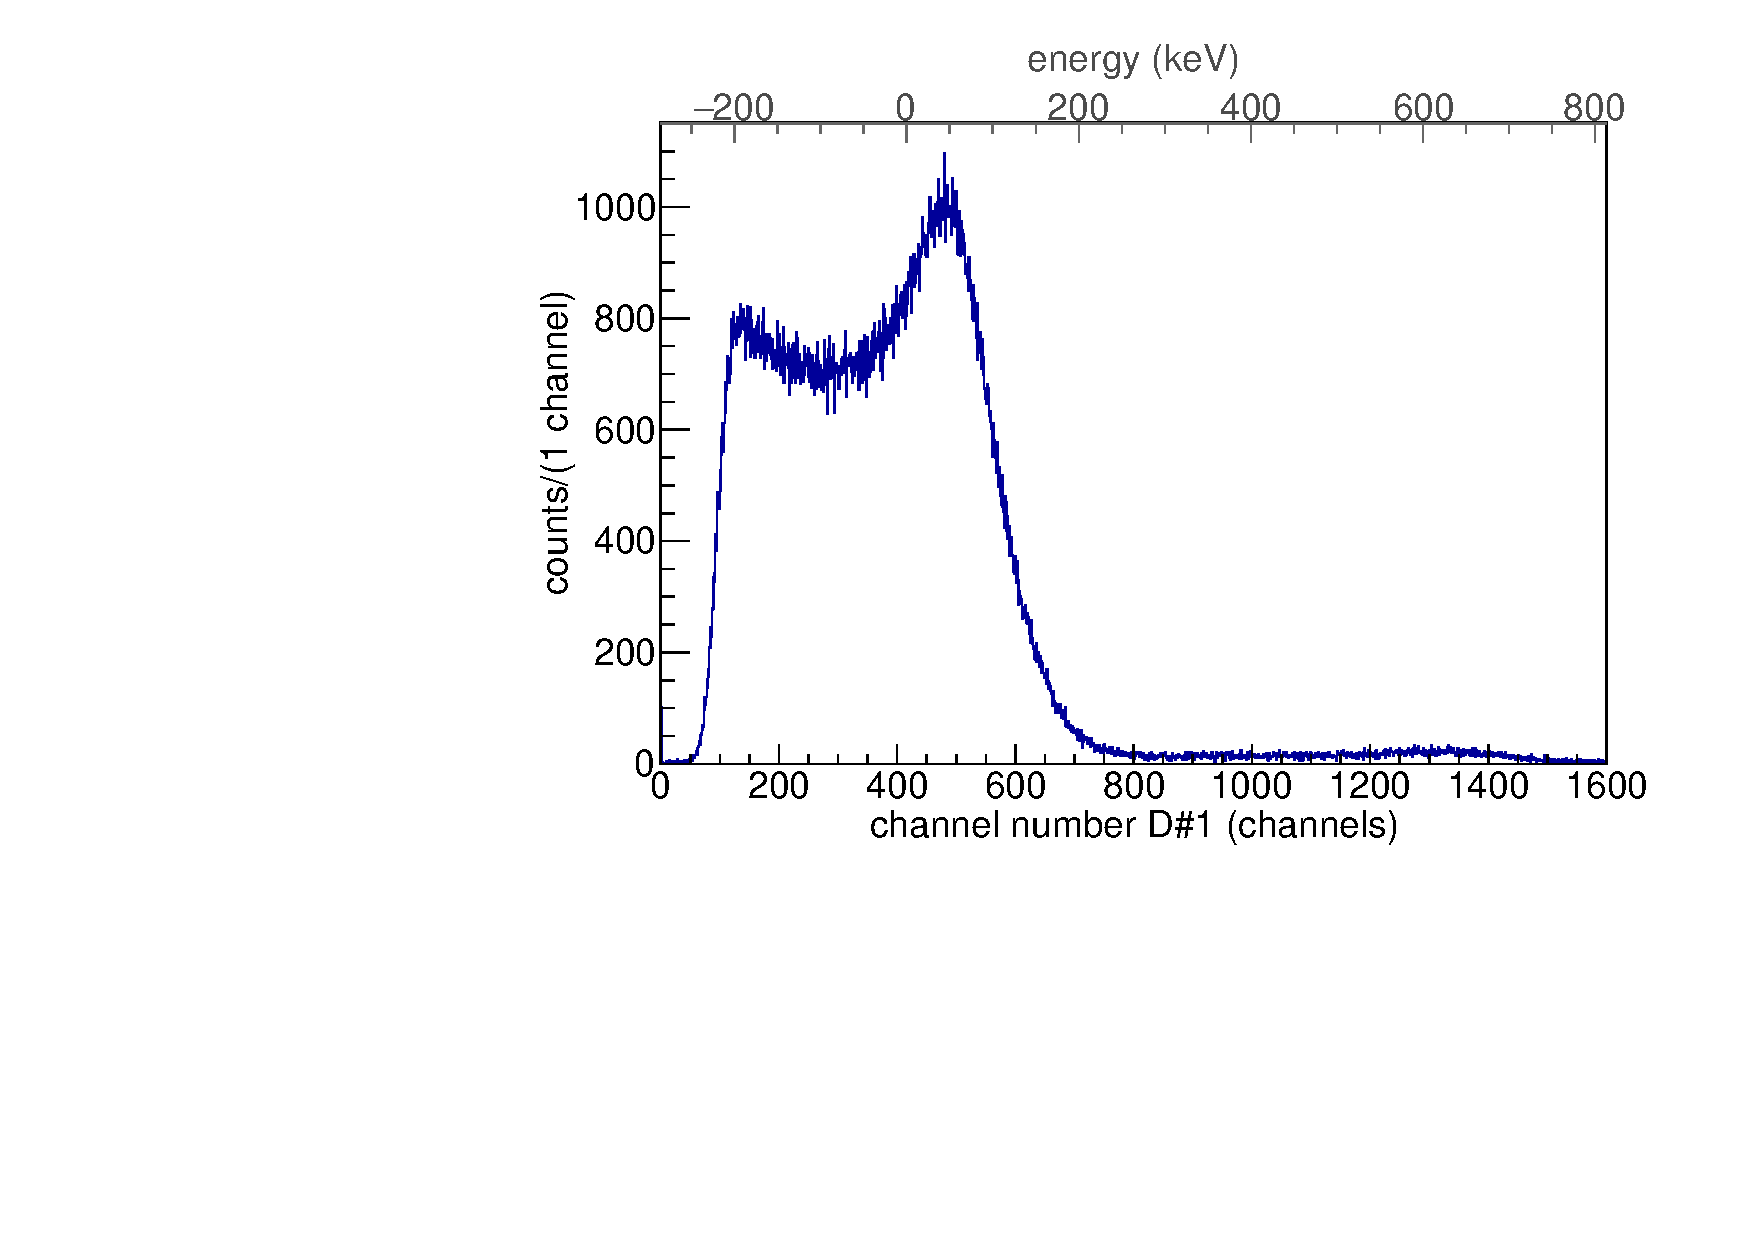
\includegraphics[width=0.4\linewidth]{digital_figures/spectrum_qlong_d1,1.pdf}
    \hspace{-0.5 cm}
    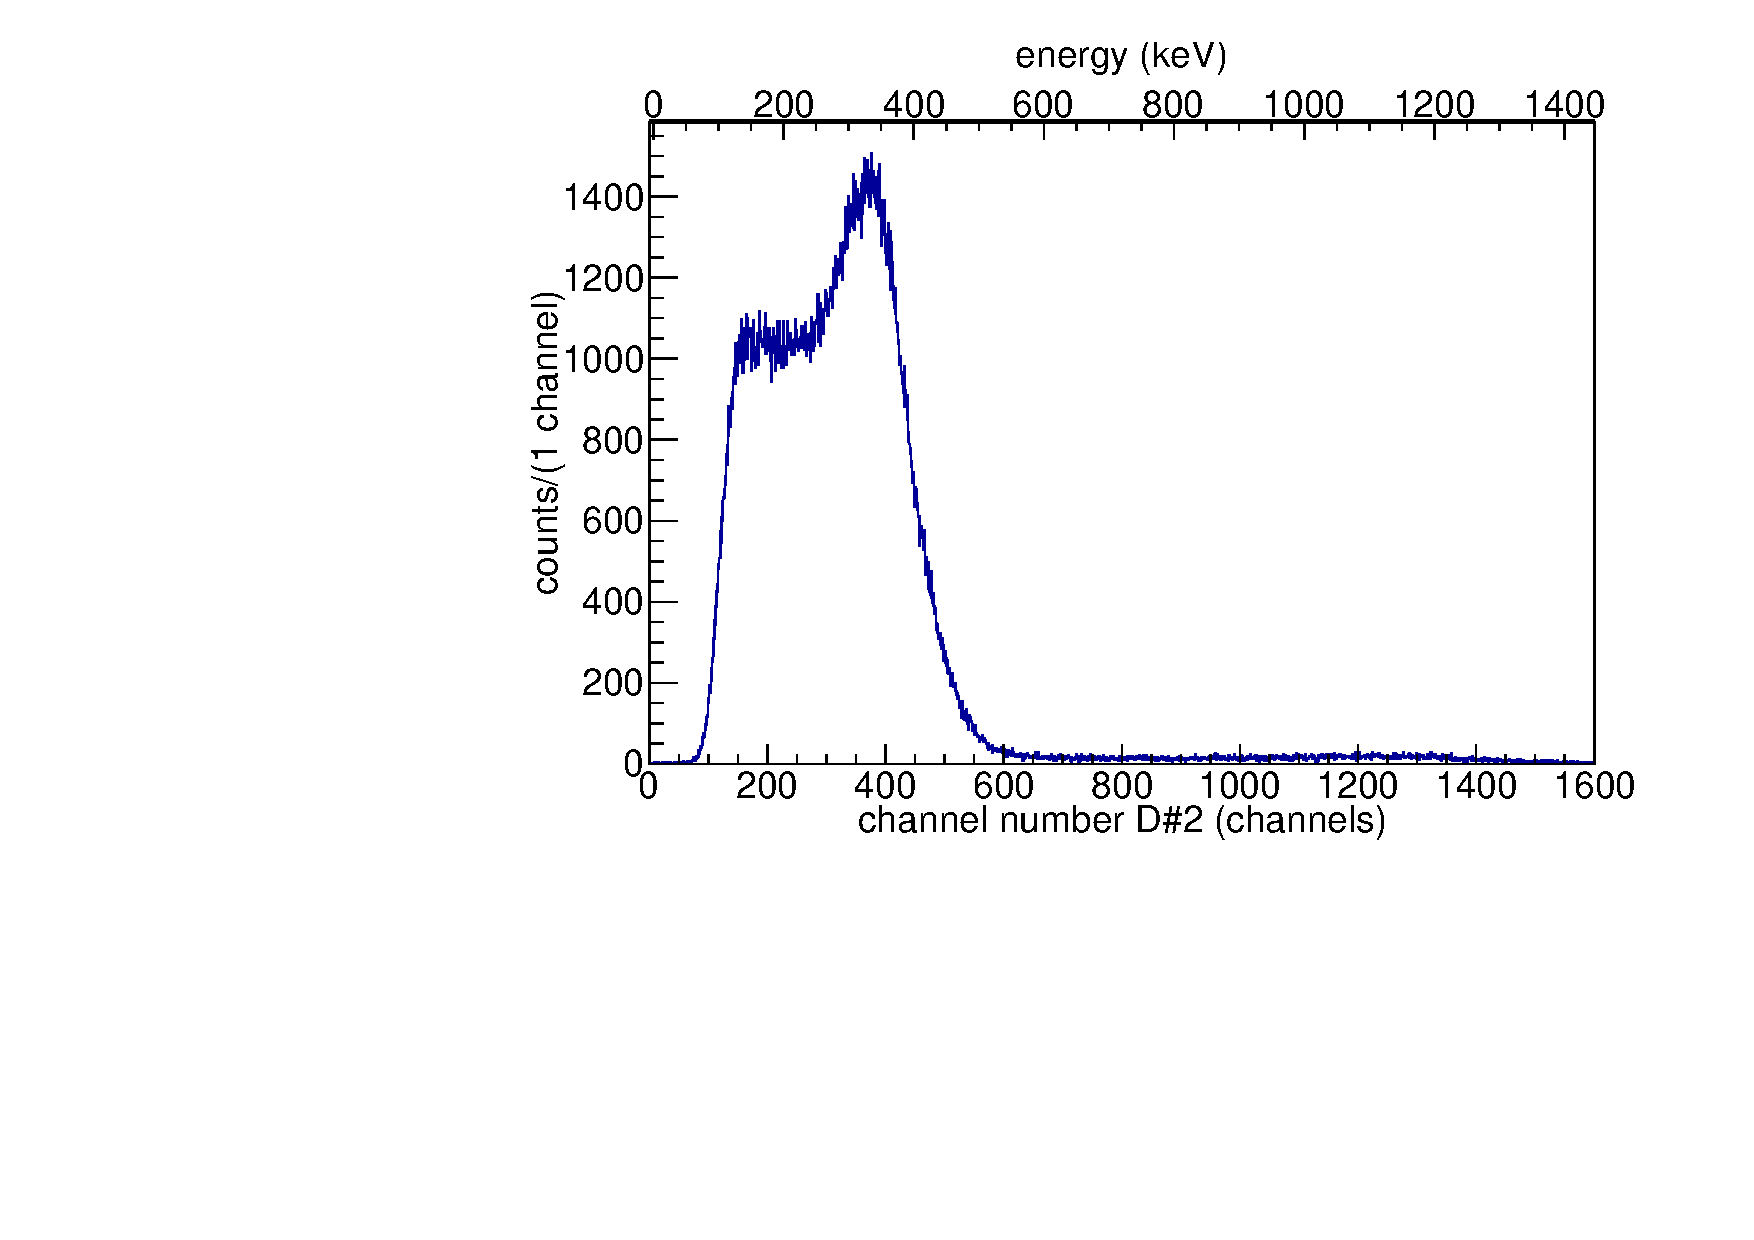
\includegraphics[width=0.4\linewidth]{digital_figures/spectrum_qlong_d2,3.pdf}

    \vspace{-0.07 cm}    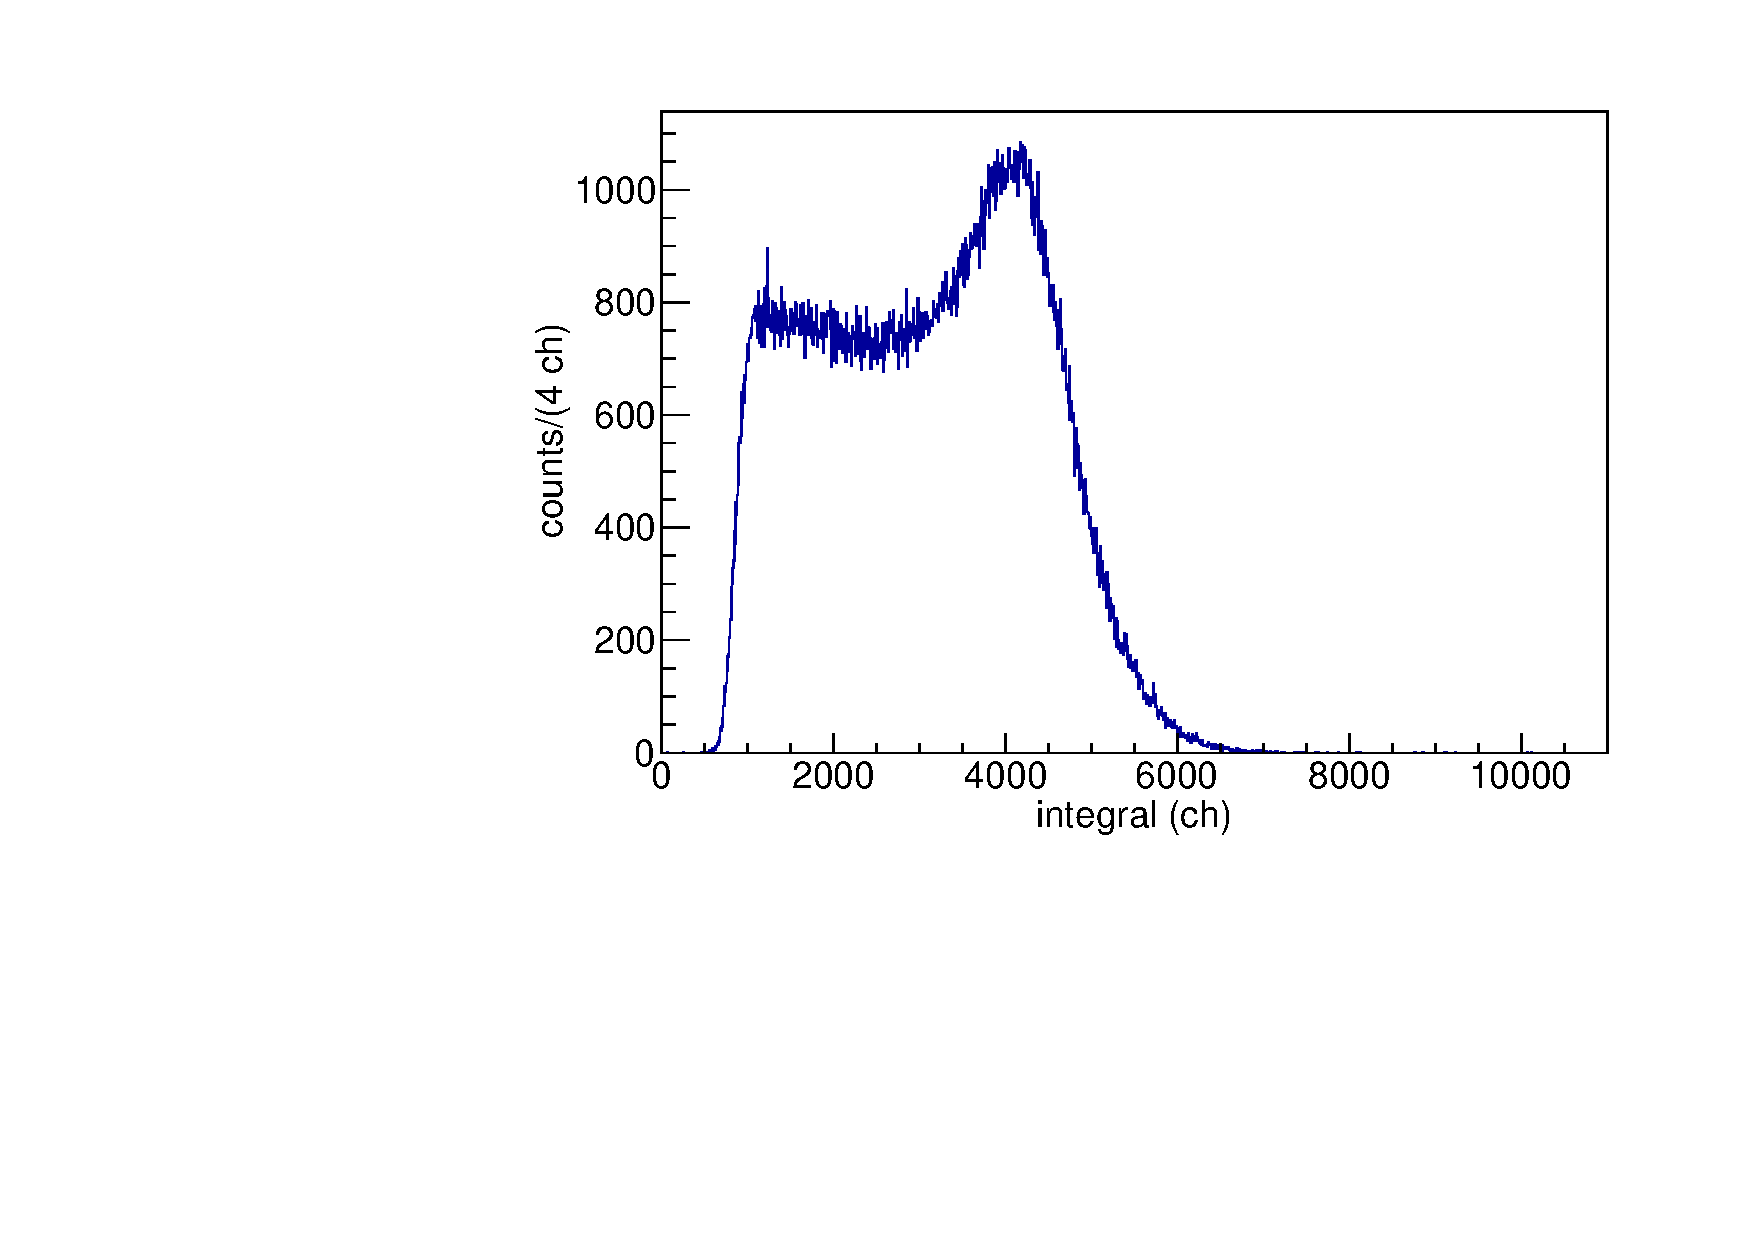
\includegraphics[width=0.4\linewidth]{digital_figures/spectrum_integral_D1.pdf}
    \hspace{-0.5 cm}
    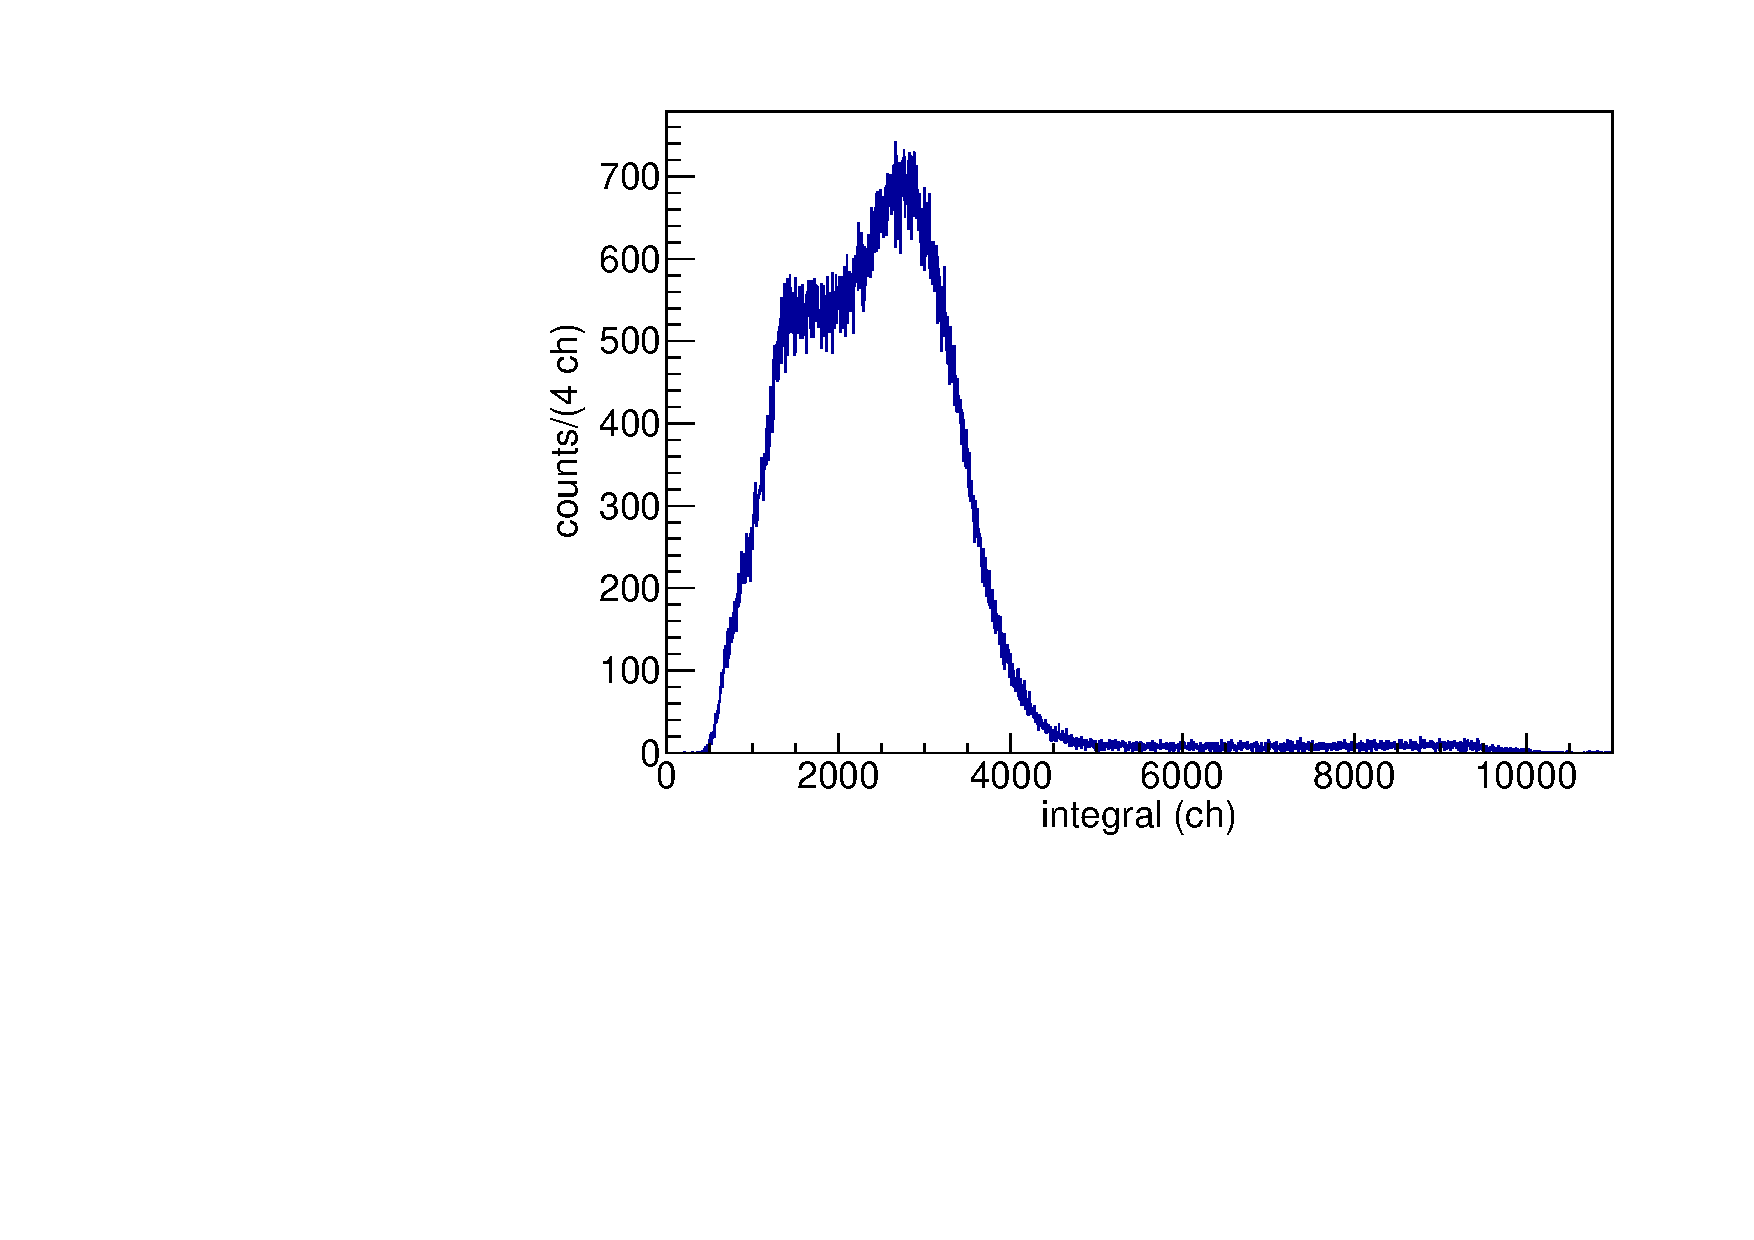
\includegraphics[width=0.4\linewidth]{digital_figures/spectrum_integral_D2.pdf}
    \vspace{-0.2 cm}
    \caption{Higher panels: energy spectra from FPGA; lower panels: energy spectra from offline integration. The panels on the left correspond to D\#1, while the panels on the right to D\#2. The energy calibration of D\#1 appears to be wrong.}
   \label{fig:energy sprectra}
\end{figure}
The resulting histograms\footnote{As mentioned above, the events registered in this section are in coincidence; as a result, in the energy spectrum only the first Compton edge is visible (related to the two in coincidence photons of energy $511\,\mathrm{keV}$).} (Fig. \ref{fig:energy sprectra}, lower panels) differ from the energy spectra obtained directly from the FPGA (Fig. \ref{fig:energy sprectra}, higher panels) in the scale of the channel numbers. 
This fact may be due to a normalization factor which was not considered in the  algorithm we used for calculating the integral.
For a given detector, the differences in the shapes of the histograms are likely to be caused by the offline integration procedure, that was not the same as the one used in the FPGA. 
Moreover, as for D\#1, the highest energy signals do not appear in the offline histogram because they were saturated, hence excluded. Finally, it may be seen clearly that the calibration of D\#1 is definitely wrong, since the position of the CE is not correct.
% In the following graphs (Fig. \ref{fig:energy spectra}), the results are already calibrated by using the energy calibration of the detectors.

% As mentioned above, the events registered in this section are in coincidence, so the only events shown in the energy spectra are related to the two in coincidence photons with energy of $511\,\mathrm{keV}$; as a result, the only visible peak is the first Compton edge (the 1275 keV CE is missing).


\subsubsection{Shaped signal}
The digital CFD is built as follows. A bipolar signal is created as the sum of two copies of the input waveform: first the signal is inverted and attenuated by a factor $f$, then it is delayed by a time $D$. An example is shown in the left panel of Fig. \ref{fig: shaped signals} for a D\#1 signal, with $D\!=\!4$ ns and $f\!=\!0.2$. 
The time that the bipolar signal crosses the zero reference level (usually the baseline) is expected to be independent of the pulse amplitude. 
The zero crossing time is calculated by interpolating between the samples immediately before and immediately after the transition across the zero reference level. 
The resulting distribution for the above mentioned parameters is presented as an example (Fig. \ref{fig: shaped signals}, right panel).
\begin{figure}[H]
    \centering
    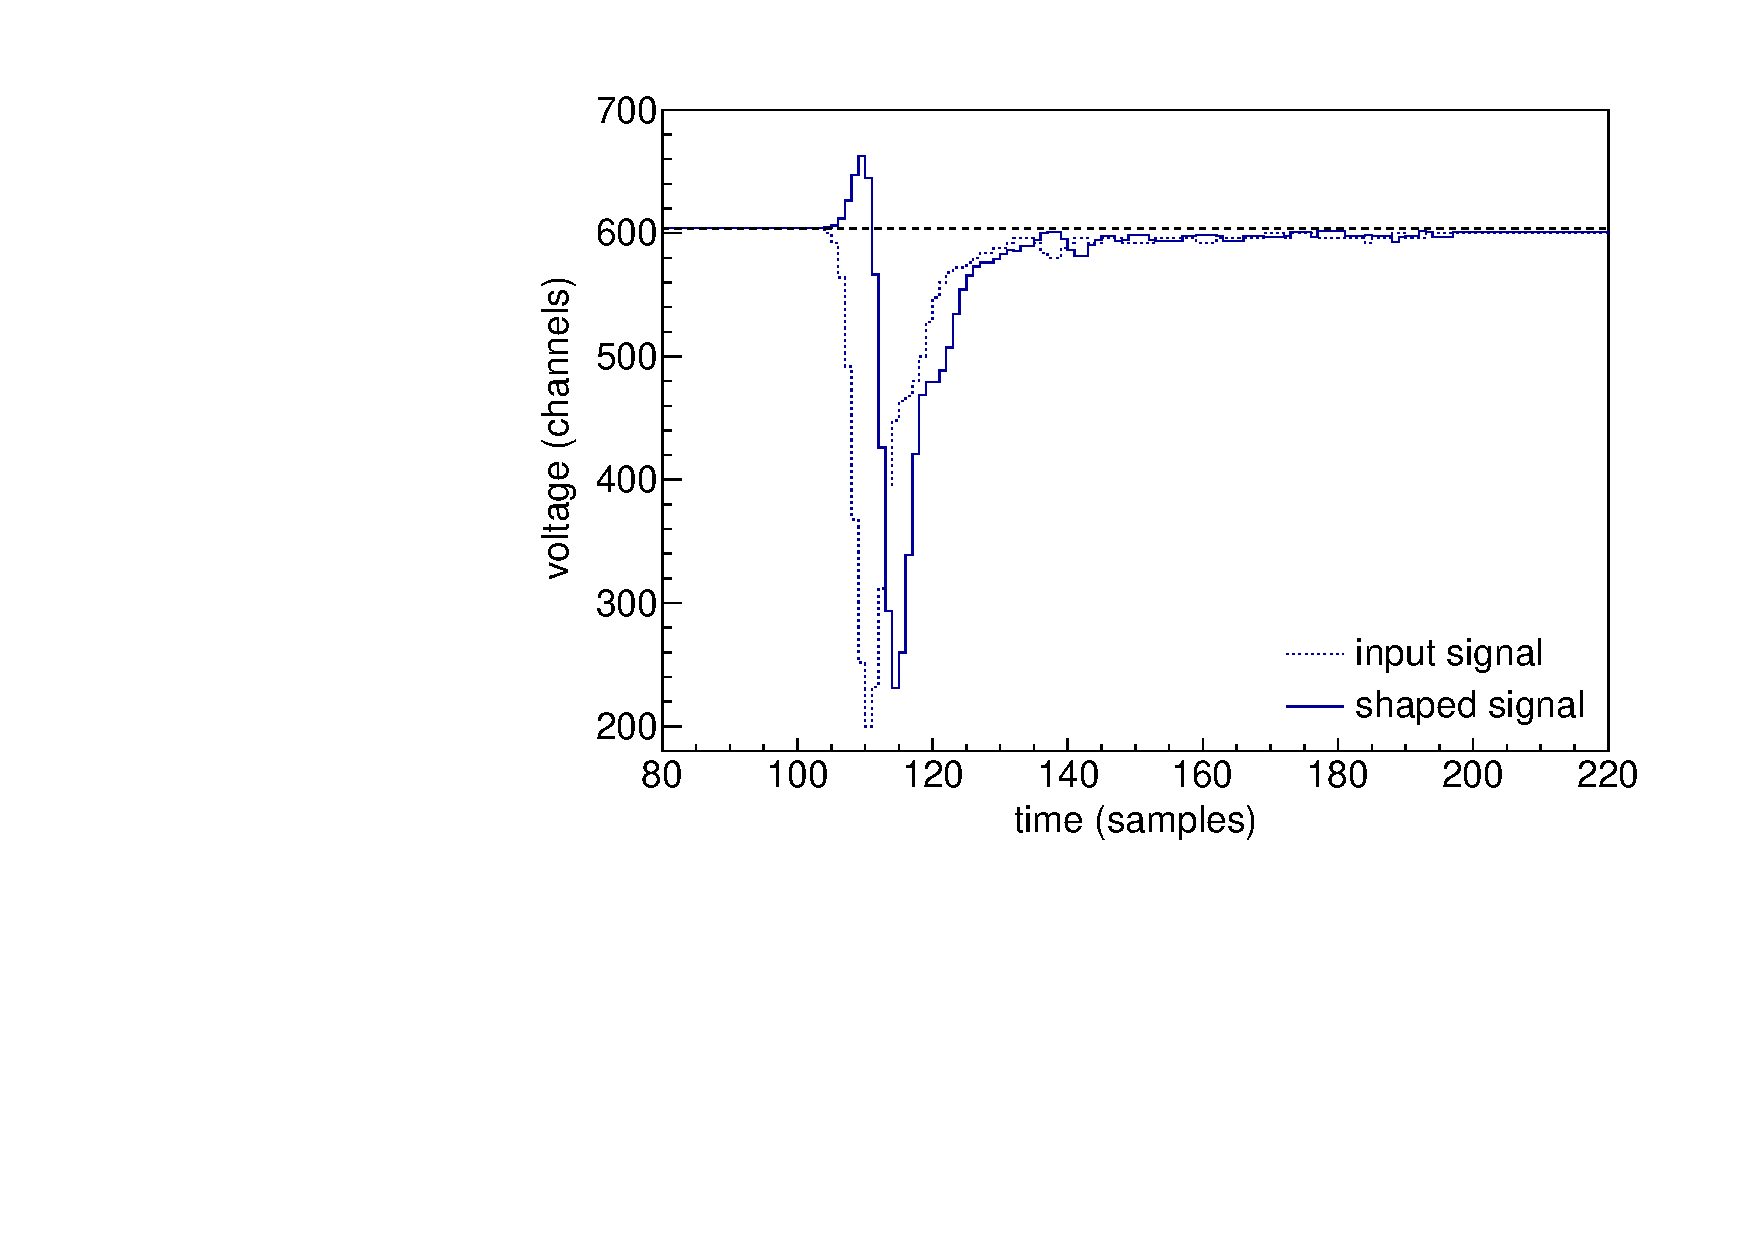
\includegraphics[scale=0.4]{digital_figures/signal7_D2_shaped.pdf}
    \hspace{-0.5 cm}
    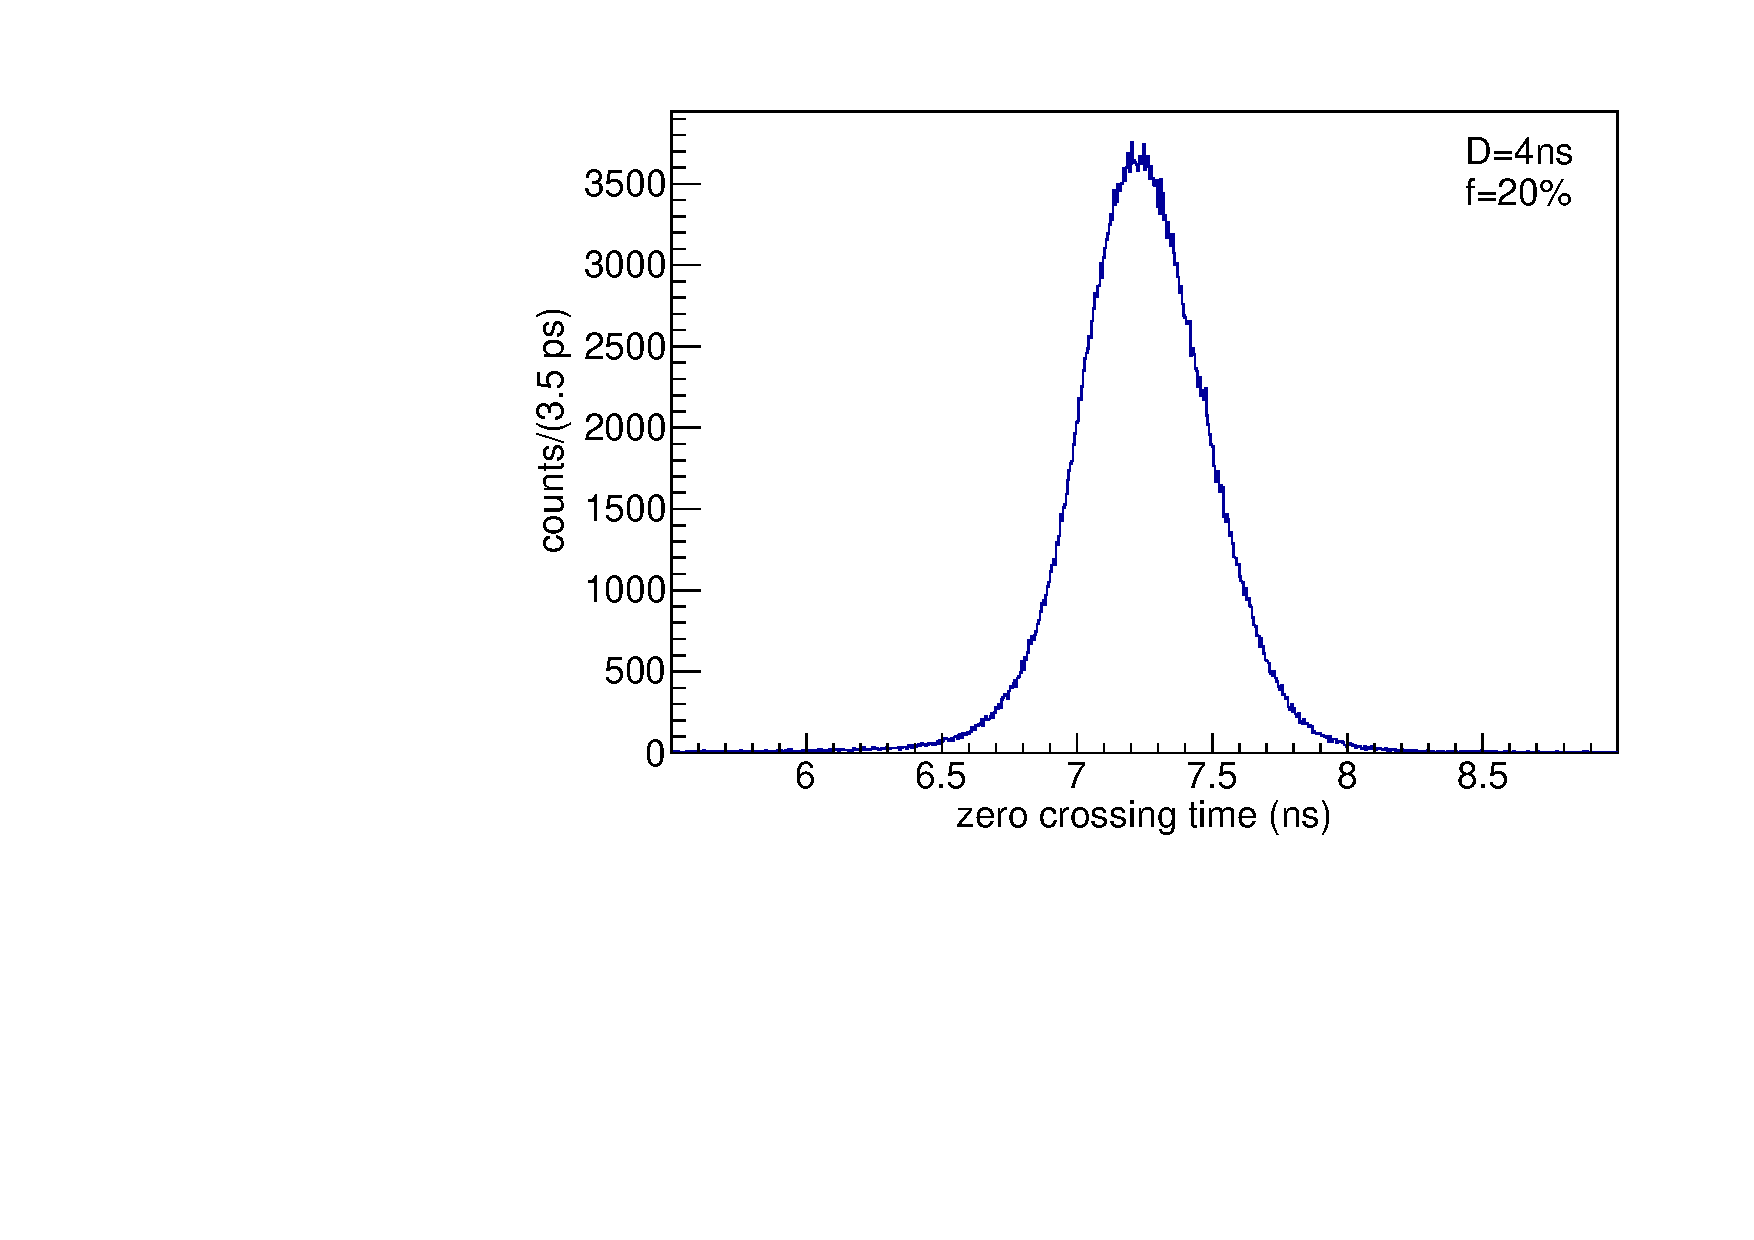
\includegraphics[scale=0.4]{digital_figures/zero_crossing_histo.pdf}
    \caption{Left panel: shaped bipolar signal for the digital CFD (D\#1, $D$=4 ns, $f$=20\%). Right panel: resulting zero crossing time distribution for the same values of $D$ and $f$.}
   \label{fig: shaped signals}
\end{figure}

\subsubsection{Time resolution as a function of the external delay and of the attenuation}
Now it is possible to study the time resolution as a function of four variables: delay $D$ and energy as in the analog processing case, and also the attenuation $f$ and the baseline estimation.
For each variable, the minimum is searched by varying the value of the studied variable while keeping the other three variables fixed.
Since it is expected to have a minimum at $D=4$ ns when $f$=0.20
% on the pair $\left(D=4\,\mathrm{ns}, f=0.20\right)$ Non sono più convinta di questa cosa
, let us begin with those variables.
%\textcolor{purple}{Since the expectation values for the positions of the minima are known for the delay and for the attenuation fraction, respectively about $4\,\mathrm{ns}$ and $0.20\%$, let us begin with those variables.}

So firstly the fraction is set at $0.20$ and the delay varies from $1$ to $10\,\mathrm{ns}$. Each point is estimated with a Gaussian fit on the time spectrum as done in the analog case, but now the spectrum is made by the zero crossing time histogram. 
The graphic on the left in Fig. \ref{fig:digital_res_1} shows clearly that the minimum value of time resolution is obtained for $D=4\,\mathrm{ns}$, then hereafter the delay is set on this value. It corresponds just to $\approx60\%$ of the measured falling time. 

The same kind of graphic, shown on the right on Fig. \ref{fig:digital_res_1}, is made for the attenuation fraction by varying it between $10\%$ and $90\%$ and the minimum here is on $20\%$, which suggests that the pair $\left(D=4\,\mathrm{ns}, f=0.20\right)$ may be a local minimum. % as expected.
\begin{figure}[H] %provvisorio
    \centering
    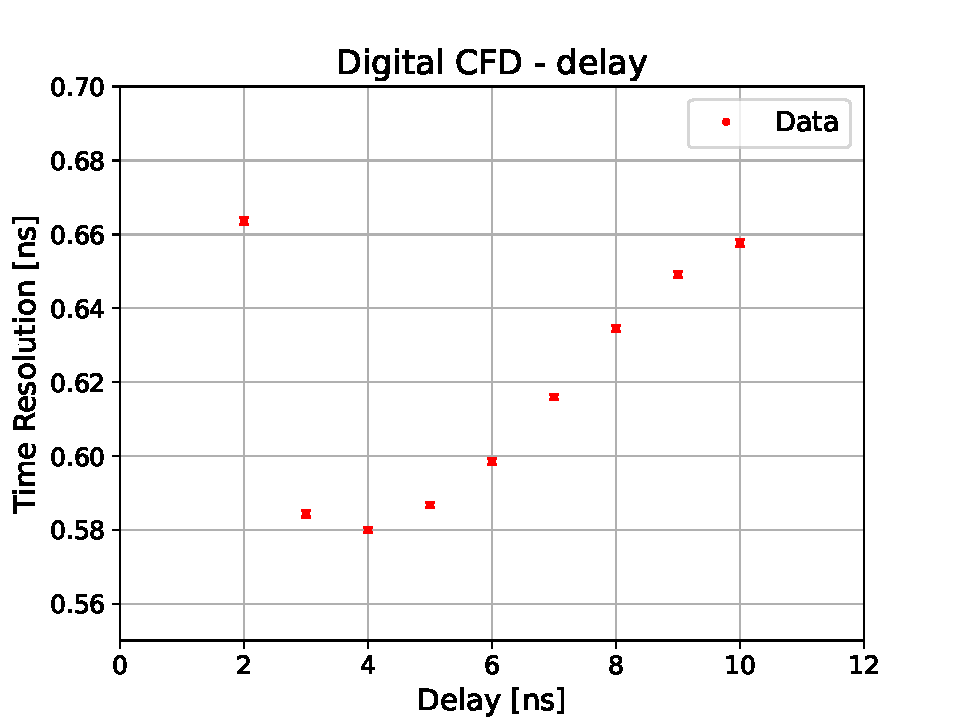
\includegraphics[width=0.48\linewidth]{digital_figures/digital_delay.pdf}
    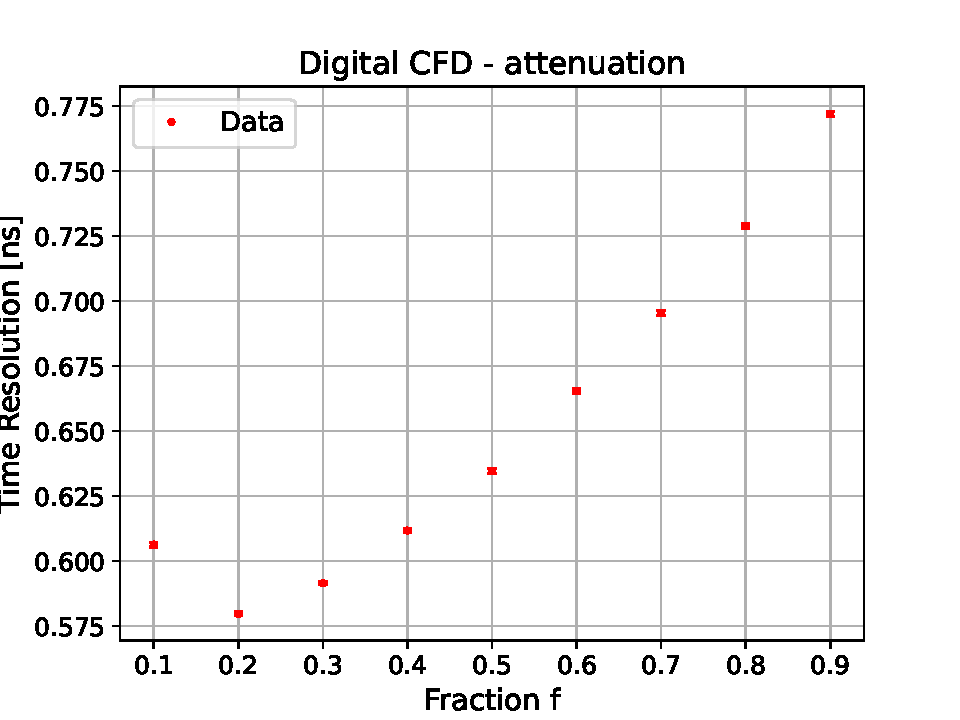
\includegraphics[width=0.48\linewidth]{digital_figures/digital_fraction.pdf}
    \caption{Time resolution as a function of the external delay with a fixed fraction $f=20\%$ (\textit{left}) and of the attenuation with a fixed delay $D=4\,\mathrm{ns}$ (\textit{right}) }
    \label{fig:digital_res_1}
\end{figure}

\subsubsection{Time resolution as a function of the energy range}\hypertarget{2.5.4}{}
As we did for the analog CFDs in section \hyperlink{2.3.4}{2.3.4}, let us now show the results of the same analysis made with the waveforms. 
At variance with the analog case, the correlation between the calibrated energy spectrum from D\#2 and the time spectrum resulting from the zero crossing time distribution (Fig. \ref{fig: digital 2D histo res vs energy}, with $D$=4 ns, $f$=20\%) displays an almost constant dependence of the coincidence peak position on the energy of the event. This means that the zero crossing time is independent of the energy to a good approximation.

Using the same lower energy thresholds and the same energy ranges up to $300\,\mathrm{keV}$ and analysing only D\#2, the graphics for the time resolution (Fig. \ref{fig: digital_energy}) were obtained: the time resolution decreases as a function of the lower energy threshold and the same effect is obtained with the addition of an upper threshold (i.e. energy range).
\begin{figure}[H]
    \centering
     \captionsetup{width=.8\linewidth}
     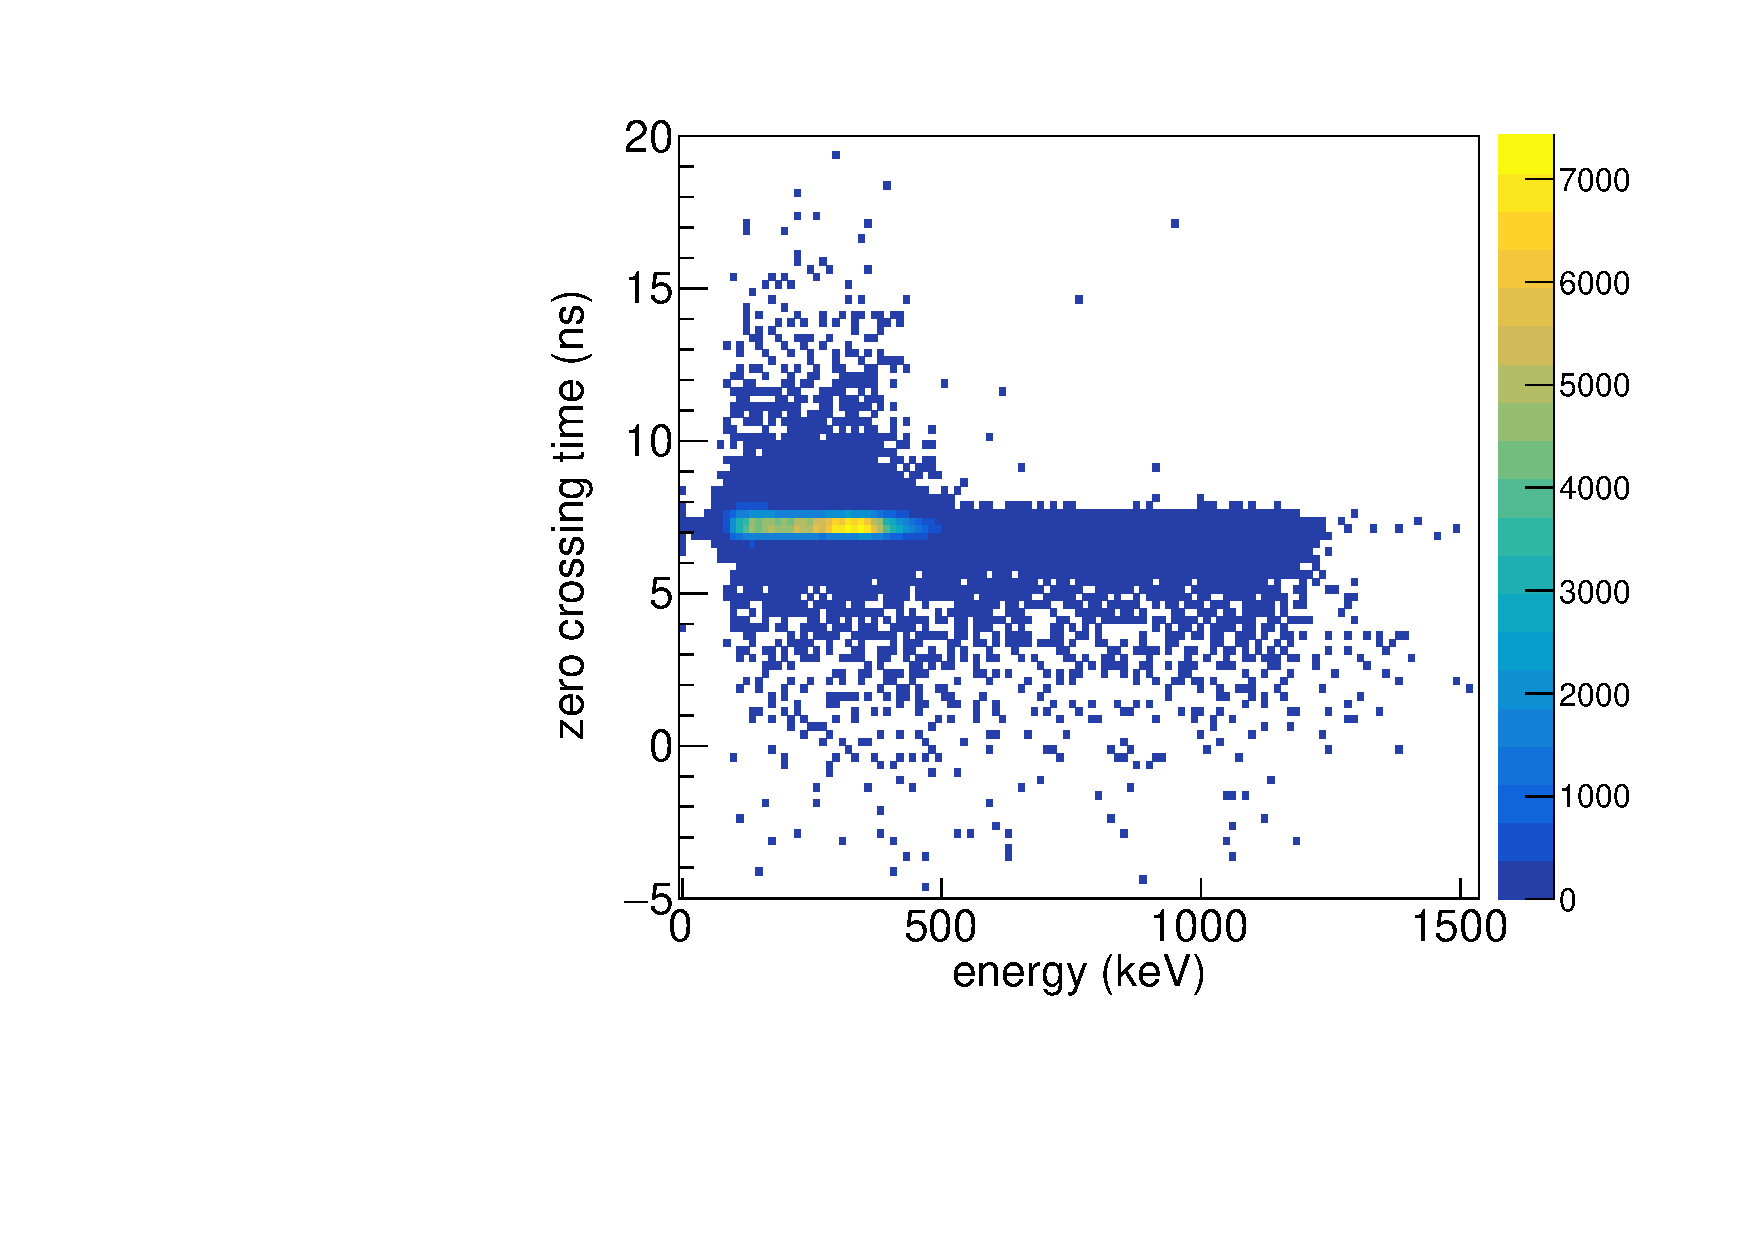
\includegraphics[scale=0.45]{digital_figures/histo2d_en.pdf}
    \caption{Correlation between the energy spectrum obtained from the FPGA for D\#2 ($x$) and the coincidence time spectrum obtained by means of the digital CFDs with $D\!=\!4$ ns and $f\!=\!0.2$ ($y$) of the \ce{^{22}Na} source. The energy axis is calibrated according to the relation found in section \ref{sect: energy calibration}.}
   \label{fig: digital 2D histo res vs energy}
\end{figure}

\begin{figure}[H]
    \centering
    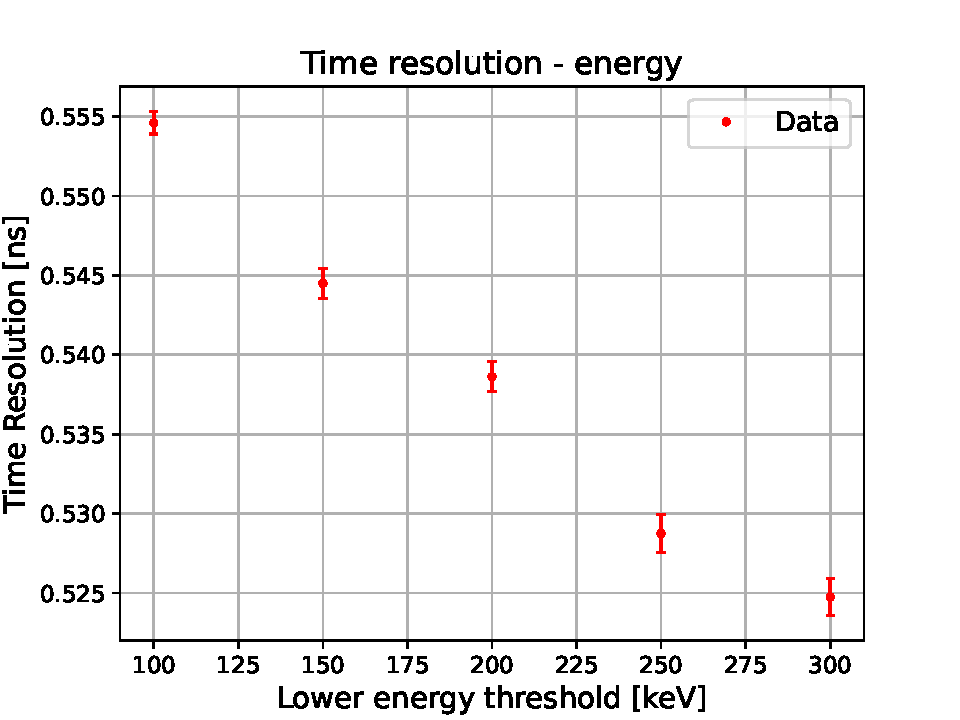
\includegraphics[width=0.48\linewidth]{digital_figures/time_res_energy_dig.pdf}
    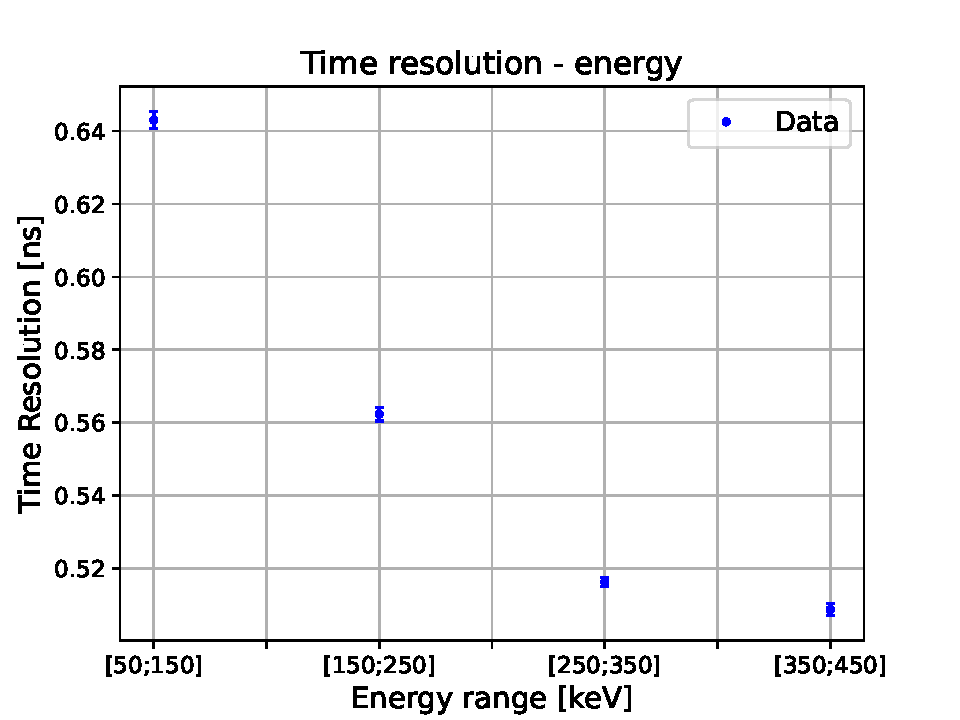
\includegraphics[width=0.48\linewidth]{digital_figures/time_res_energy_dig2.pdf}
    \caption{Time resolution as a function of the lower energy threshold (\textit{on the left}) and as a function of the energy range (\textit{on the right}) for $D\!=\!4$ ns and $f\!=\!0.2$}
    \label{fig: digital_energy}
\end{figure}

\subsubsection{Time resolution as a function of the baseline}
Until now, the zero reference value to identify the crossing of the bipolar signal was equal to the evaluated baseline, which is different event by event. 
In this last section this value will be changed and the time resolution will be studied again. 
In particular, the aim is to check if there is an optimal value implying the lowest time resolution. Let us consider a variation of $\pm2$ channels and $\pm1$ channel around the mean value of the baselines %$bl_0$ for 
of D\#1 events ($\approx603.5$ ch) and then, separately, around the one of 
% $bl_1$ for 
D\#2 events ($\approx858.5$ ch). 
The results on Fig. \ref{fig: baseline} do not display any significant influence on the time resolution.

\begin{figure}[H]
    \centering
    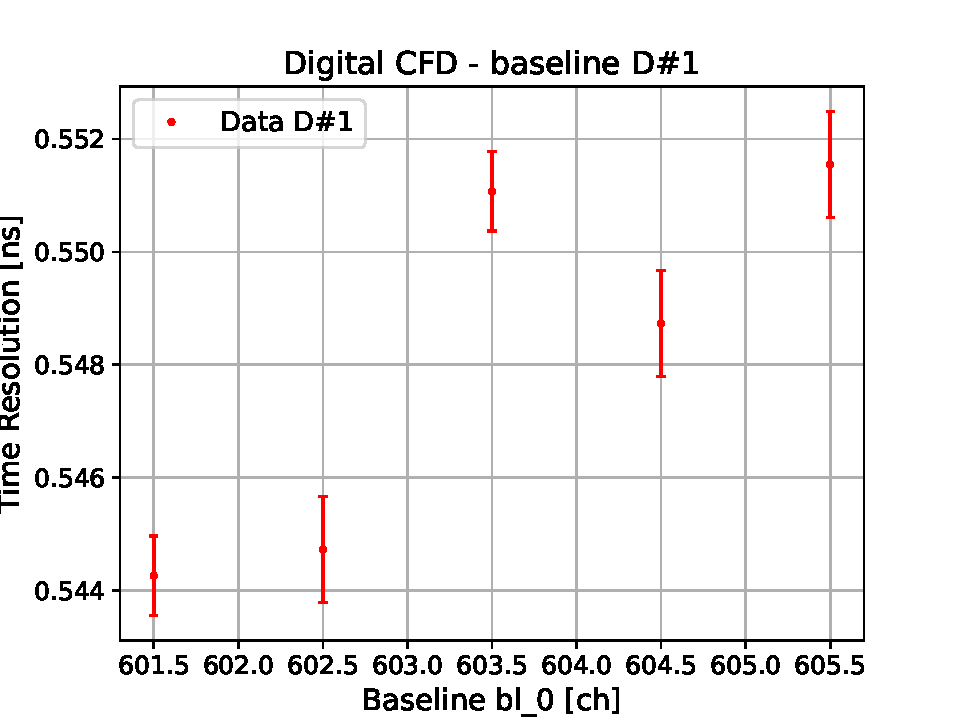
\includegraphics[width=0.48\linewidth]{digital_figures/digital_bl0.pdf}
    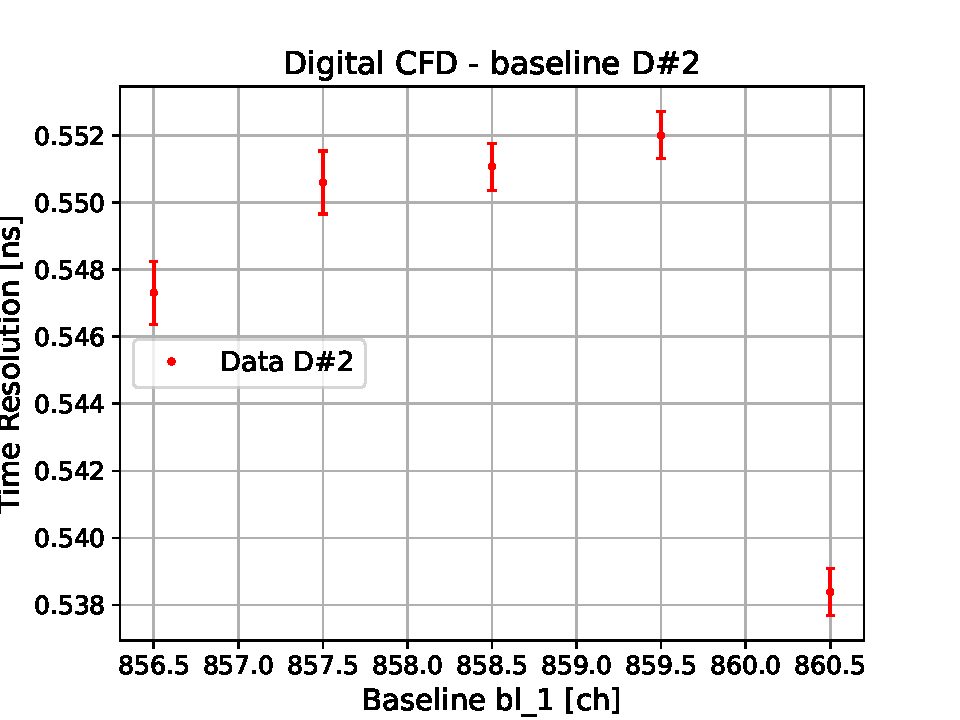
\includegraphics[width=0.48\linewidth]{digital_figures/digital_bl1.pdf}
    \caption{Time resolution as a function of the baseline value for each detector, D\#1 on the left and D\#2 on the right. }
    \label{fig: baseline}
\end{figure}


\section{Conclusions}\label{sect:conclusions}
\hypertarget{3}{}

\paragraph{Study of the time resolution} The main analysis of this experiment was dedicated to the study the time resolution. This first goal was pursued by looking for the optimal parameters that influence the timing measurement and by comparing the results with the expected values. The analysis was done firstly in the analog case and then by means of the digitized signals.

\begin{itemize}
    \item [-] \textbf{Study of time resolution as a function of external delay and comparison with digital results}: 
    % with the available data, recorded at the laboratory, 
    having calibrated in time the output of the TAC and having estimated the delay introduced by a LEMO cable, 
    it was possible to verify a minimum around the expected external delay of about $4$ to $5\,\mathrm{ns}$, considering the falling time of the signal discussed in the first \hyperlink{2.1}{section}. As regards the minimum, a similar result was obtained with the digital analysis. However, the minimum resolution achieved with the digital analysis is significantly better than the analog one: ($R_{\mathrm{dig}}\simeq0.58\,\mathrm{ns}$ against $R_{\mathrm{ana}}\simeq1.05\,\mathrm{ns}$ ).
    
     \item [-]  \textbf{Study of the time resolution as a function of the energy for analog and digital CFDs}: 
     for the analog CFD the time resolution turned out to decrease with the energy threshold until a minimum in
     % was achieved for a lower energy threshold on 
     the interval $\left[750;\,900\right]\, \mathrm{keV}$; 
    it also decreases as a function of the energy range.
    % and for a energy range around $900\,\mathrm{keV}$. 
    Time resolution studied with digital signals decreases up to $300\,\mathrm{keV}$, both for the lower energy threshold and the energy range conditions. Like in the external delay case, the best time resolution has been achieved with the digital analysis. 

    \item [-] \textbf{Study of the time resolution as a function of the attenuation and of the baseline by means}: the attenuation has been studied on a range of $\left[0.1;\,0.9\right]$ with the external delay fixed at $4$ ns and shows a minimum at the value of $0.20$ as expected. The baseline was studied around the mean value, but it shows up not to have a clear trend to define the optimization of this value to get a better time resolution.

\end{itemize}

\noindent With respect to the difference between time resolution values for analog CFD and digital CFD, let us point out that there was an asymmetry in the TAC spectra of the analog CFDs, in particular the left side was higher, both in the study as a function of the delay and of the energy. 


\paragraph{Result: speed of light} The last goal of the analysis was the calculation of the speed of light using coincidence photons with different time of arrivals. For this part, the parameters, in particular the slope, of the TAC calibration were used. The result $c=(2.80\pm0.03)\cdot 10^8 \, \mathrm{m/s}$
 is not compatible with the known value and it is affected by a systematic error as discussed in the dedicated \hyperlink{2.4}{section}.
 
\paragraph{Remarks} The analysis on this report revealed some possible systematic errors about D\#1, whose energy calibration was not correct. The reason may be related to the settings of the digitizer or of the first acquisition data. Another problem related to D\#1 concerns the baseline of the waveforms that is particularly low with respect to that of D\#2. %should be around $800-900\,\mathrm{mV}$.\\
Besides, a further analysis can be done by implementing the ROOT macro in order to have a multivariate function %fit 
to study the time resolution as a function of the delay and the attenuation.


\end{document}